\documentclass[11pt]{article}
\usepackage[english]{babel}
\usepackage{minted}
\usepackage{amsmath}
\usepackage{amsthm}
\usepackage{graphicx}
\usepackage{subcaption}
\usepackage{booktabs}
\usepackage[utf8]{inputenc}
% More styles for bullets
\usepackage{pifont}
\usepackage[left=25mm, top=25mm, bottom=30mm, right=25mm]{geometry}
\usepackage[colorlinks=true, linkcolor=blue, urlcolor=cyan]{hyperref}
\usepackage[style=authoryear-ibid,backend=biber,maxbibnames=99,maxcitenames=2,uniquelist=false,isbn=false,url=true,eprint=false,doi=true,giveninits=true,uniquename=init]{biblatex} % Allows you to do citations - does Harvard style and compatible with Zotero
\newcommand\titleofdoc{Assignment 3}
\newcommand\GroupName{Machine Learning}
\begin{document}
\begin{center}
        \vspace*{2cm} % Adjust spacings to ensure the title page is generally filled with text

        \Huge{\titleofdoc} 
            
        \vspace{2 cm}
        \Large{\GroupName}
       
        \vspace{0.25cm}
        \large{Yuyutsu Saini}
       
        \vspace{3 cm}
        \Large{$28^{th}$ October, $2022$}
        
        \vspace{0.25 cm}
        \Large{COL 774: Machine Learning}
\end{center}
\vspace{1cm}
\tableofcontents

\section{Decision Trees, Random Forests and Gradient Boosted Trees}

We will be using Na\"{i}ve Bayes approach to classify the text in one of the two categories i.e. review being negative and positive. Here, Our assumption is occurrence of a word in a review is conditionally independent of occurrence of another word. All precision, recall and f1 scores are on test data for different features taken for training the model.



\subsection{Dataset 1: Mammographic mass lesion severity prediction}
Mammography is the most effective method for breast cancer screening available today.
We will work on a mammography dataset available from the
UCI repository.The dataset contains 5 features: (a) BI-RADS assessment \\
(b) Age \\ (c) Shape \\ (d) Margin \\ (e) Density \\ \\
The Decision Tree is implemented using this dataset to predict the type of brease cancer.

\subsubsection{Decision Tree Construction and Visualization}
The missing data in this part is just ignored and deafault parameters are used. The observations made are:
\begin{enumerate}
\item Depth of decision tree obtained are : 20
\item No. of leaves in decision tree obtained are : 119
\item Accuracy over Training data set = 0.9692307692307692
\item Accuracy over Validation data set = 0.8016528925619835
\item Accuracy over Test data set = 0.7272727272727273
\end{enumerate}

% \paragraph{Decision Tree Plot}
% \\
\begin{figure}[H]
  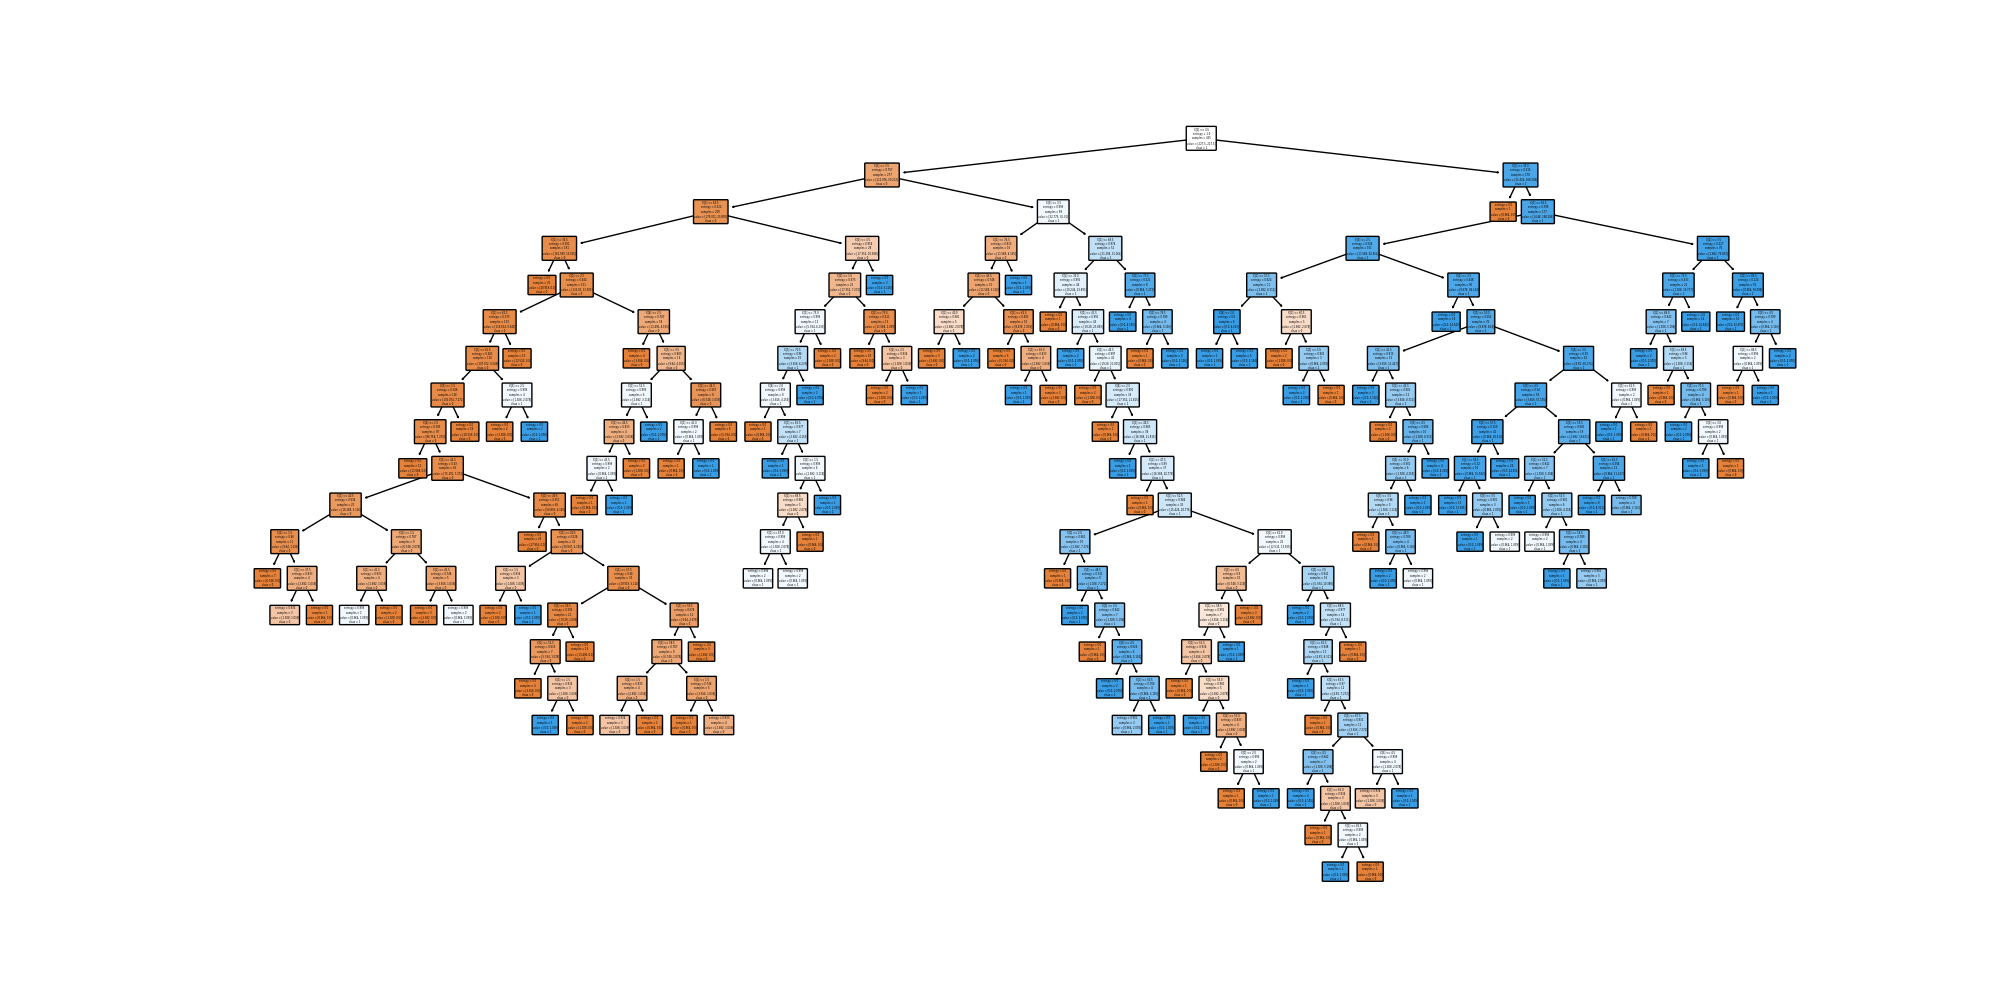
\includegraphics[width=\linewidth]{1_a_decision_tree.png}
  \caption{Decision Tree}
  \label{fig1A}
\end{figure}
On the training set, the model clearly shows an overfit, which leads to excellent training accuracy but subpar performance on the test set.
\subsubsection{Decision Tree Grid Search}
Here in this part the grid search over the space of parameters including max depth, min samples split and min samples leaf is performed. The set of parameters of over which grid search is performed are:
\begin{itemize}
\item n$\_$estimators : [10,20,40,50],  
\item subsample : [0.1,0.2,0.3,0.4,0.5,0.6], 
\item max$\_$depth : [4,5,6,7,8,9,10]
\end{itemize}
\hline
\vspace{3mm}
The observations made are:
\begin{enumerate}
\item Depth of decision tree obtained are : 5
\item No. of leaves in decision tree obtained are : 18
\item Accuracy over Training data set after Grid search = 0.8637362637362638
\item Accuracy over Validation data set after Grid search = 0.8760330578512396
\item Accuracy over Test data set after Grid search = 0.7865612648221344
\end{enumerate}
\begin{figure}[H]
  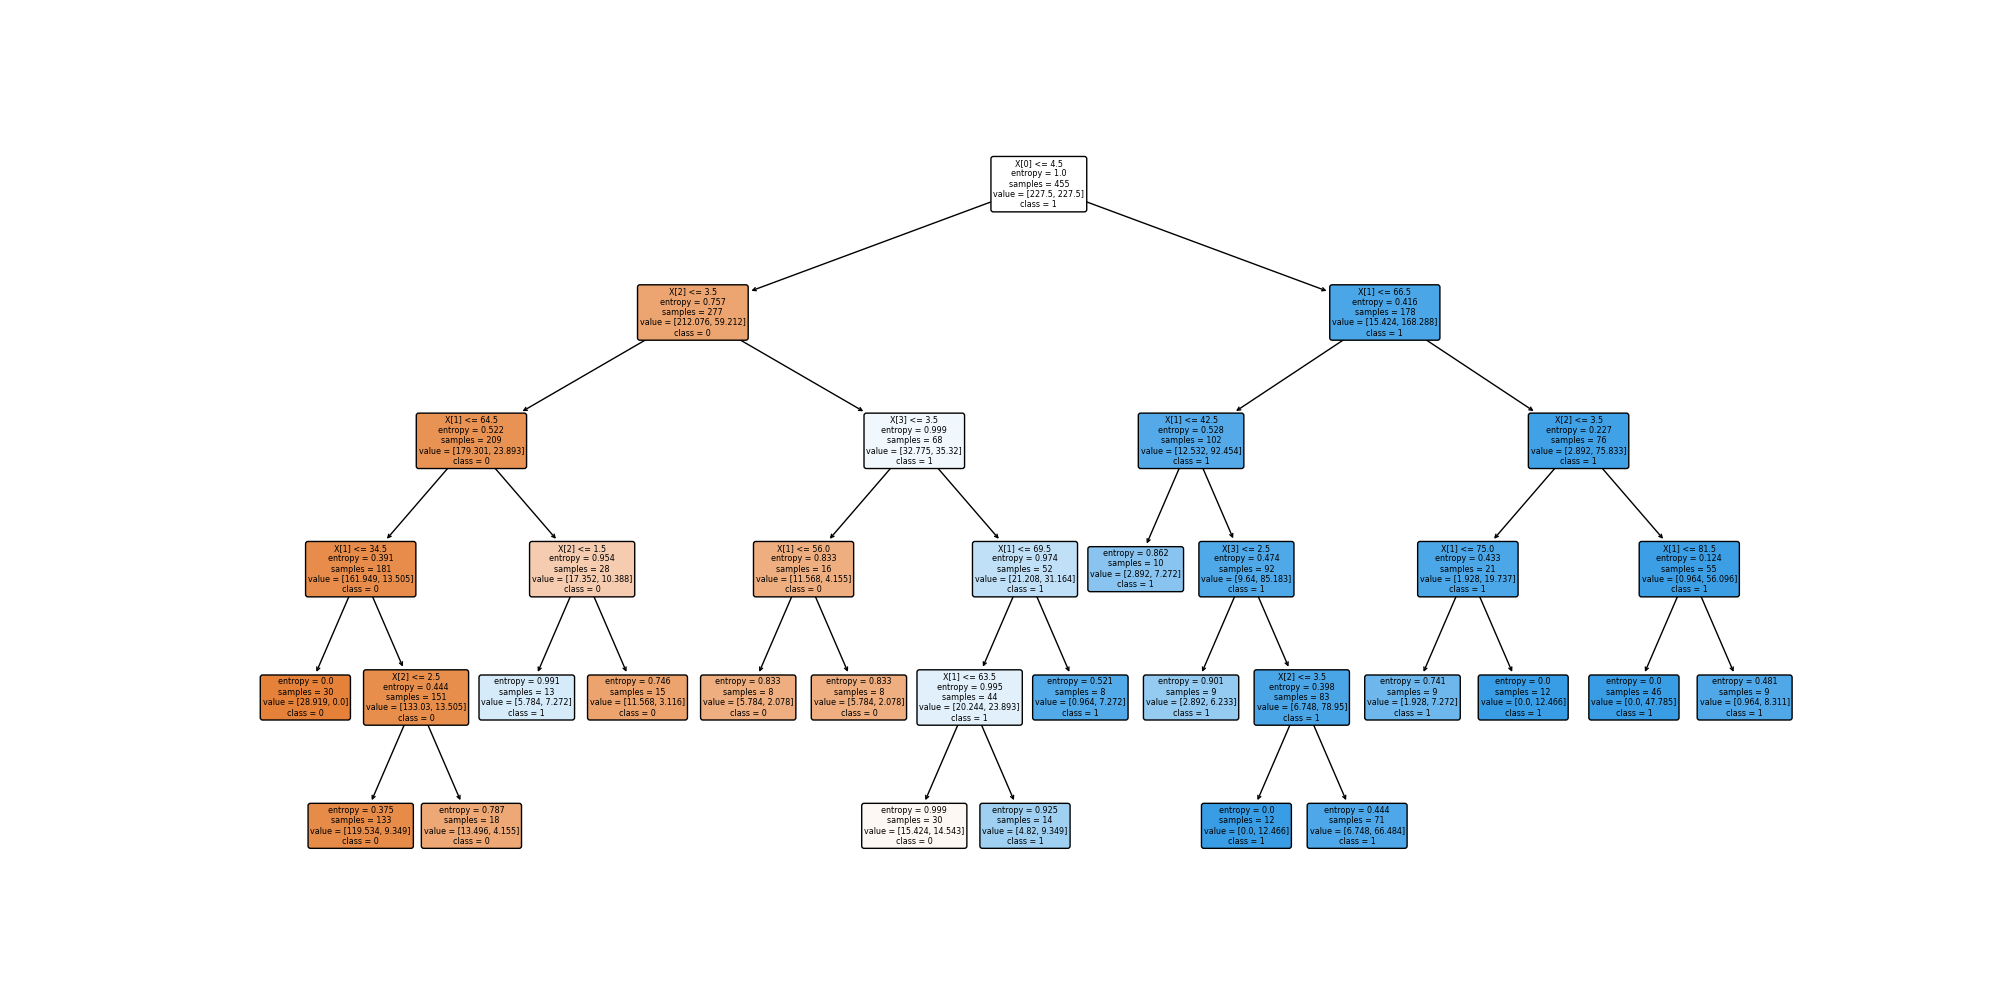
\includegraphics[width=\linewidth]{1_b_Best_decision_tree.png}
  \caption{Decision Tree}
  \label{fig1B}
\end{figure}
By varying and adjusting the parameters of decision tree classifier, we have prevented overfitting to some extent.
\subsubsection{Decision Tree Post Pruning (Cost Complexity Pruning)}
Minimal cost complexity pruning is implemented using DecisionTreeClassifier.cost$\_$complexity$\_$pruning$\_$path. Pruning was performed on the default decision tree using scikit-learn to obtain a range of ccp alpha parameters and corresponding impurities. The variation in parameters with ccp alpha was observed and plotted. The last ccp alpha value corresponding to a trivial single-node tree was included just for mentioning the existence of single node.
\begin{enumerate}
\item Depth of decision tree obtained are : 3
\item No. of leaves in decision tree obtained are : 4
\item Accuracy over Training data set after Pruning = 0.8395604395604396
\item Accuracy over Validation data set after Pruning = 0.9090909090909091
\item Accuracy over Test data set after Pruning = 0.7905138339920948
\end{enumerate}
\begin{figure}[H]
  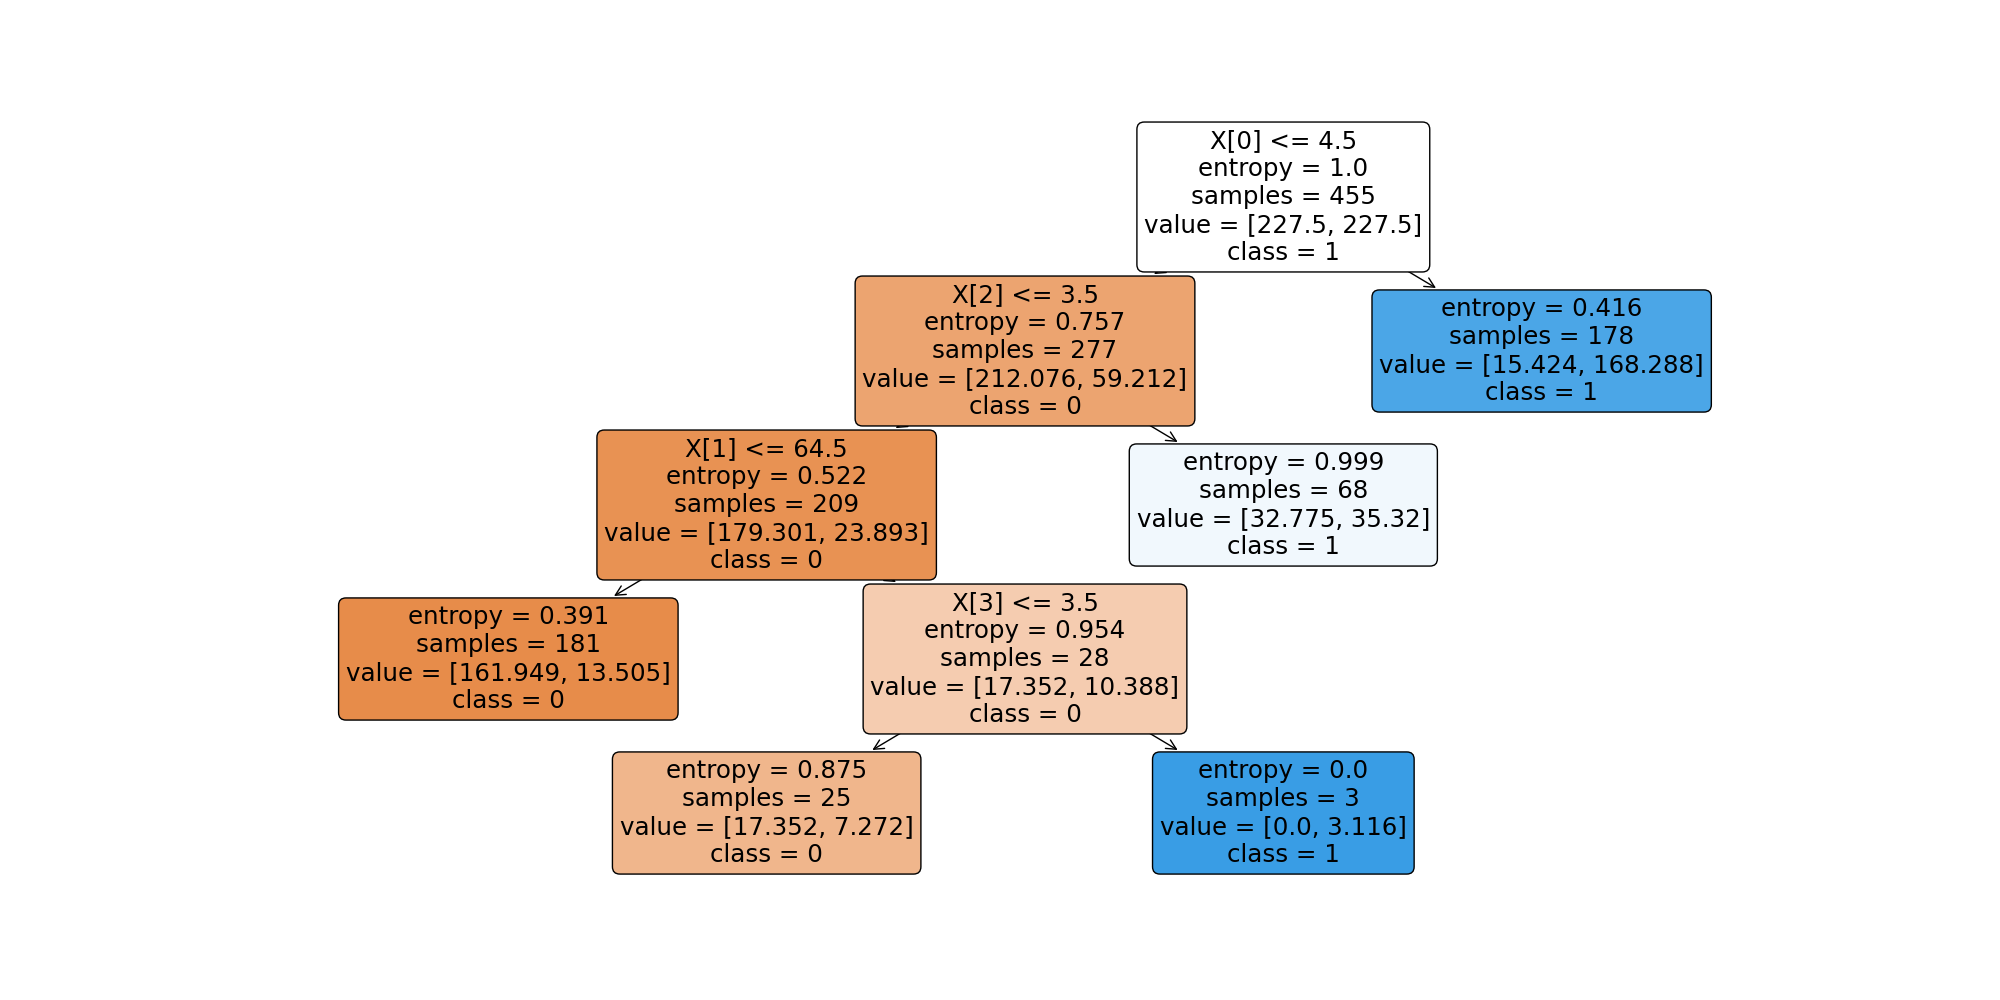
\includegraphics[width=\linewidth]{1_c_Best_pruned_tree.png}
  \caption{Decision Tree}
  \label{fig1B}
\end{figure}
\begin{figure}[H]
  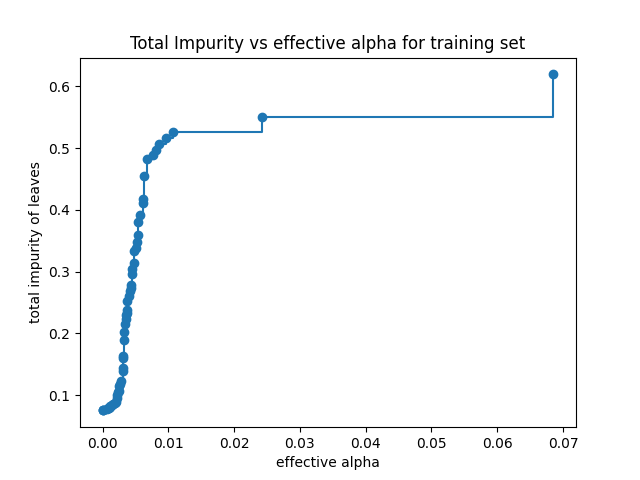
\includegraphics[width=\linewidth]{1_c_impurity_vs_alpha.png}
  \caption{Impurity Vs Alpha}
  \label{fig1B}
\end{figure}
\begin{figure}[H]
  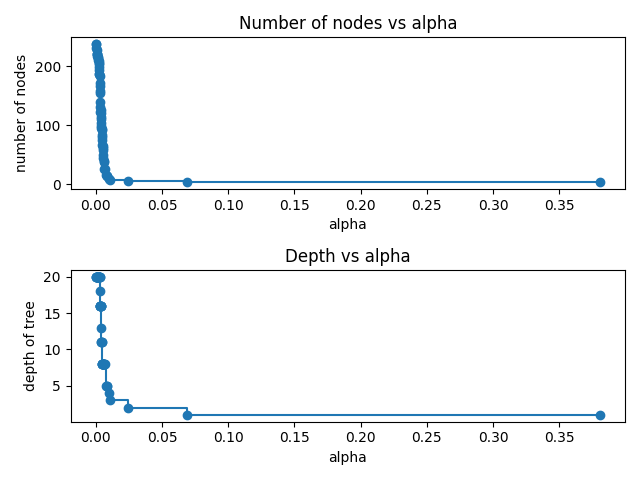
\includegraphics[width=\linewidth]{1_c_nodeVsAlpha__depthVsAlpha.png}
  \caption{Nodes and Depth Vs Alpha}
  \label{fig1B}
\end{figure}
\begin{figure}[H]
  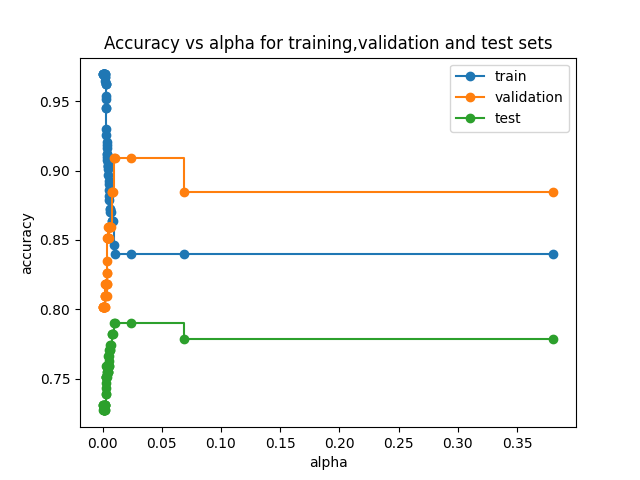
\includegraphics[width=\linewidth]{1_c_Accuracy.png}
  \caption{Accuracy}
  \label{acc}
\end{figure}
Figure \ref{acc} shows the increase in validation and test set accuracies along with decline in the training set accuracies. Here, pruning prevents overfitting and as a result the training set accuracy decreases. But, at higher values of ccp alphas the model underfits and training, validation, test set accuracies decreases.
\subsubsection{Random Forests}
% \subsubsection{Decision Tree Post Pruning (Cost Complexity Pruning)}
The Random Forest is implemented after performing grid search over :\\
(a) n estimators \\
(b) max features \\ (c) min sample split \\
And, the out of bag accuracy is used here. The Accuracy over the best classifier build using grid search over random forest is:
\begin{enumerate}
\item Out of Bad Accuracy is = 0.8351648351648352
\item Accuracy over Training data set after using random forest = 0.8857142857142857
\item Accuracy over Validation data set after using random forest = 0.9173553719008265
\item Accuracy over Test data set after using random forest = 0.802608695652174
\end{enumerate}
The random forest slightly increases the accuracy by a small amount on all three data sets.
\subsubsection{Missing Data Imputation}
\textbf{The Accuracy over the best classifier build using grid search over Decision Tree is:}
\begin{enumerate}
\item Imputation used over training data for decision tree is : median
\item Depth of decision tree obtained are : 18
\item No. of leaves in decision tree obtained are : 155
\item Accuracy over Training data set = 0.9608938547486033
\item Accuracy over Validation data set = 0.8347107438016529
\item Accuracy over Test data set = 0.7470355731225297
\end{enumerate}
The above results shows that with imputation by median, the model learns more about the trend of the data and tries to conserve the distribution and hence performs significantly better than the case where these data points
were ignored.
\vspace{3mm}
\hline

\begin{enumerate}
\item Imputation used over training data for decision tree is : mode
\item Depth of decision tree obtained are : 16
\item No. of leaves in decision tree obtained are : 155
\item Accuracy over Training data set = 0.9590316573556797
\item Accuracy over Validation data set = 0.8264462809917356
\item Accuracy over Test data set = 0.7509881422924901
\end{enumerate}
Here also, with imputation the model learns more about the data and performs better than ignoring the data points with missing attributes. The mode imputation results in better performance on the test and validation dataset.
\vspace{3mm}
\hline
\vspace{3mm}
\textbf{The Accuracy over the best classifier build using grid search over Random Forest is:}
\begin{enumerate}
\item Accuracy over Training data set after using imputation in Random Forest as median = 0.88268156424581
\item Accuracy over Validation data set after using imputation in Random Forest as median = 0.9090909090909091
\item Accuracy over Test data set after using imputation in Random Forest as median = 0.7984189723320159
\end{enumerate}
\hline
\begin{enumerate}
\item Accuracy over Training data set after using imputation in Random Forest as mode = 0.8752327746741154
\item Accuracy over Validation data set after using imputation in Random Forest as mode = 0.9090909090909091
\item Accuracy over Test data set after using imputation in Random Forest as mode = 0.8023715415019763
\end{enumerate}
Here, not much difference is made by imputation in both cases namely median and mode.
\subsubsection{ Gradient Boosted Trees}
XGBoost (Extreme Gradient Boosting) is functional gradient
boosting based approach where an ensemble of “weak learners” (decision trees in our case) is used with the goal to construct a model with less bias, and better predictive performance. I have used the XGBoost classifier
and experimenting with different parameter values (in the given range): \\ (a) n estimators (10 to 50
in range of 10) \\ (b) subsample (0.1 to 0.6 in range of 0.1) \\ (c) max depth(4 to 10 in range of 1) \\
The Accuracy obtained is:
\begin{enumerate}
\item Accuracy over Training data set after using xgb = 0.8747252747252747
\item Accuracy over Validation data set after using xgb = 0.9256198347107438
\item Accuracy over Test data set after using xgb = 0.782608695652174
\end{enumerate}
\begin{enumerate}
\item Accuracy over Training data set after using imputation in Random Forest as mode = 0.8752327746741154
\item Accuracy over Validation data set after using imputation in Random Forest as mode = 0.9090909090909091
\item Accuracy over Test data set after using imputation in Random Forest as mode = 0.8023715415019763
\end{enumerate}

\subsection{Dataset 2: Drug rating prediction}
Thus dataset related to prediction of rating associated medical
drugs, where the attributes are primarily textual. Any dataset with text attributes requires conversion of text to numerical attributes for computations to be performed. In this dataset there are two text attibutes, namely conditon and review. The review attribute contains reviews about drugs collected from patients with specified conditions. We are going to use these two text attributes to predict the rating of a drug. Here, CountVectorizer is used and punctuations and stopwords have been removed.
\subsubsection{Decision Tree Construction}
The Observations made are:
\begin{enumerate}
\item Time to train the Decision Tree : 164.48403000831604
\item Depth of decision tree obtained are : 108
\item No. of leaves in decision tree obtained are : 45268
\item Accuracy over Training data set = 1.0
\item Accuracy over Validation data set = 0.5603546260513753
\item Accuracy over Test data set = 0.5565599077483911
\end{enumerate}
\subsubsection{Decision Tree Grid Search}
Here in this part the grid search over the space of parameters
including max depth, min samples split and min samples leaf is performed. The set of parameters of over which grid search is performed are:
\begin{itemize}
\item n$\_$estimators : [100],  
\item max$\_$features : [1], 
\item min$\_$samples$\_$split : [2],
\item max$\_$leaf$\_$nodes : [None]
\end{itemize}
\hline
\vspace{3mm}
The observations made are:
\begin{enumerate}
\item Time to train the Decision Tree using grid search : 883.0011687278748
\item Depth of decision tree obtained are : 108
\item No. of leaves in decision tree obtained are : 45312
\item Accuracy over Training data set after Grid search = 1.0
\item Accuracy over Validation data set after Grid search = 0.5604579553204241
\item Accuracy over Test data set after Grid search = 0.5584942156753339
\end{enumerate}
Here, the grid search is made over the small dataset because it was taking lots and lots of time to grid search over a range of parameters.
\subsubsection{Decision Tree Post Pruning (Cost Complexity Pruning)}
Pruning was performed on the default decision tree using scikit-learn to obtain a range of \texttt{ccp\_alpha} parameters and corresponding impurities. No. of \texttt{ccp\_alpha} obtained were 32k. The variation in parameters with \texttt{ccp\_alpha} was observed and plotted. The last ccp\_alpha value corresponding to a trivial single-node tree was excluded for analysis. For the selection of the best model, every $100^{th}$ value in \texttt{ccp\_alpha} was used to train and validate considering the huge number of values. \\
\\
The best classifier was selected by performance on validation set and the following results were obtained.
\begin{enumerate}
\item The \texttt{ccp\_alpha} obtained is : 0.0
\item Depth of decision tree obtained are : 108
\item No. of leaves in decision tree obtained are : 45312
\item Accuracy over Training data set after Grid search = 1.0
\item Accuracy over Validation data set after Grid search = 0.5704278543261246
\item Accuracy over Test data set after Grid search = 0.5693974656758163
\end{enumerate}
\subsubsection{Random Forests}
In this part, a grid search was performed on the hyperparameters \texttt{n\_estimators}, \texttt{min\_samples\_split} and \texttt{max\_features} in order to train random forest. \\
\\
The parameters and accuracies obtained is:
\begin{enumerate}
\item n$\_$estimators : 450
\item max$\_$features : 0.8
\item min$\_$sample$\_$split : 2
\item The out of bag accuracy is : 65.2035749574238162
\item Accuracy over Training data set after Grid search = 1.0
\item Accuracy over Validation data set after Grid search = 0.6494551836124622
\item Accuracy over Test data set after Grid search = 0.6471878656758163
\end{enumerate}
When using a random forest instead of a single decision tree, we see a considerable improvement in test accuracy since random forests have less volatility and are thus more resilient. The training accuracy still shows overfitting, which gradient boosting may help to reduce.
\subsubsection{Gradient Boosted Trees (XGBoost)}
Extreme gradient boosting based estimators were constructued using the \textit{xgoost} package and grid search was performed to tune it's hyperparameters. \\
\\
The parameters and accuracies obtained is:
\begin{enumerate}
\item n$\_$estimators : 450
\item max$\_$depth : 40
\item min$\_$sample$\_$split : 2
% \item The out of bag accuracy is : 65.2035749574238162
\item Accuracy over Training data set after Grid search = 0.7789541967642131
\item Accuracy over Validation data set after Grid search = 0.5273314397721642
\item Accuracy over Test data set after Grid search = 0.5341263645122973
\end{enumerate}
The training, test and validation set accuracies decreases because the no. of trees are less.
\subsubsection{GBM (Gradient Boosted Machines)}
Gradient boosted machines based estimators were constructued using the \textit{lightgbm} package and grid search was performed to tune it's hyperparameters.\\
\\
The parameters and accuracies obtained is:
\begin{enumerate}
\item n$\_$estimators : 2000
\item max$\_$depth : 40
\item subsamples : 0.4
% \item The out of bag accuracy is : 65.2035749574238162
\item Accuracy over Training data set after Grid search = 0.9856419676425406
\item Accuracy over Validation data set after Grid search = 0.6491883246014102
\item Accuracy over Test data set after Grid search = 0.6413071624533165
\end{enumerate}
LightGBM performs the best among all the preceding models because to the scalability to huge datasets of gradient boosted machines, with a noticeable decrease in overfit on training set as compared to the random forest model in section.\\
\\
The decision tree models train noticeably quicker than the other models outlined above, with pruning and parameter fixing requiring almost the same amounts of time while taking somewhat longer than the default decision tree. The multi-estimator models that perform the slowest with parameter fixing are random forest and XGBoost, respectively. LightGBM performs better on the test data and achieves training speeds that are comparable to those of a decision tree.
\subsubsection{Training with Varying amount of data}
\begin{enumerate}
    \item The training data set size is 20000.
    \item Part A : Training Accuracy : 1.0, Test Accuracy : 0.32, Validation Accuracy : 0.32
    \item Part B : Training Accuracy : 1.0, Test Accuracy : 0.32, Validation Accuracy : 0.32
    \item Part C : Training Accuracy : 1.0, Test Accuracy : 0.32, Validation Accuracy : 0.32
    \item Part D : Training Accuracy : 1.0, Test Accuracy : 0.32, Validation Accuracy : 0.32
    \item Part E : Training Accuracy : 0.98, Test Accuracy : 0.28, Validation Accuracy : 0.28
    \item Part F : Training Accuracy : 1.0, Test Accuracy : 0.33, Validation Accuracy : 0.32
\end{enumerate}
\hline
\begin{enumerate}
    \item The training data set size is 40000.
    \item Part A : Training Accuracy : 1.0, Test Accuracy : 0.38, Validation Accuracy : 0.37
    \item Part B : Training Accuracy : 1.0, Test Accuracy : 0.38, Validation Accuracy : 0.39
    \item Part C : Training Accuracy : 1.0, Test Accuracy : 0.38, Validation Accuracy : 0.38
    \item Part D : Training Accuracy : 1.0, Test Accuracy : 0.38, Validation Accuracy : 0.37
    \item Part E : Training Accuracy : 0.94, Test Accuracy : 0.36, Validation Accuracy : 0.36
    \item Part F : Training Accuracy : 0.99, Test Accuracy : 0.39, Validation Accuracy : 0.38
\end{enumerate}
\hline
\begin{enumerate}
    \item The training data set size is 60000.
    \item Part A : Training Accuracy : 1.0, Test Accuracy : 0.41, Validation Accuracy : 0.41
    \item Part B : Training Accuracy : 1.0, Test Accuracy : 0.42, Validation Accuracy : 0.42
    \item Part C : Training Accuracy : 1.0, Test Accuracy : 0.41, Validation Accuracy : 0.40
    \item Part D : Training Accuracy : 1.0, Test Accuracy : 0.40, Validation Accuracy : 0.41
    \item Part E : Training Accuracy : 0.83, Test Accuracy : 0.43, Validation Accuracy : 0.43
    \item Part F : Training Accuracy : 0.98, Test Accuracy : 0.45, Validation Accuracy : 0.45
\end{enumerate}
\hline
\begin{enumerate}
    \item The training data set size is 80000.
    \item Part A : Training Accuracy : 1.0, Test Accuracy : 0.49, Validation Accuracy : 0.49
    \item Part B : Training Accuracy : 1.0, Test Accuracy : 0.50, Validation Accuracy : 0.51
    \item Part C : Training Accuracy : 1.0, Test Accuracy : 0.50, Validation Accuracy : 0.50
    \item Part D : Training Accuracy : 1.0, Test Accuracy : 0.51, Validation Accuracy : 0.50
    \item Part E : Training Accuracy : 0.78, Test Accuracy : 0.53, Validation Accuracy : 0.52
    \item Part F : Training Accuracy : 0.97, Test Accuracy : 0.54, Validation Accuracy : 0.54
\end{enumerate}
\hline
\begin{enumerate}
    \item The training data set size is 100000.
    \item Part A : Training Accuracy : 1.0, Test Accuracy : 0.55, Validation Accuracy : 0.55
    \item Part B : Training Accuracy : 1.0, Test Accuracy : 0.55, Validation Accuracy : 0.56
    \item Part C : Training Accuracy : 1.0, Test Accuracy : 0.55, Validation Accuracy : 0.55
    \item Part D : Training Accuracy : 1.0, Test Accuracy : 0.54, Validation Accuracy : 0.54
    \item Part E : Training Accuracy : 0.75, Test Accuracy : 0.55, Validation Accuracy : 0.55
    \item Part F : Training Accuracy : 0.97, Test Accuracy : 0.56, Validation Accuracy : 0.55
\end{enumerate}
\hline
\begin{enumerate}
    \item The training data set size is 120000.
    \item Part A : Training Accuracy : 1.0, Test Accuracy : 0.51, Validation Accuracy : 0.51
    \item Part B : Training Accuracy : 1.0, Test Accuracy : 0.52, Validation Accuracy : 0.51
    \item Part C : Training Accuracy : 1.0, Test Accuracy : 0.52, Validation Accuracy : 0.52
    \item Part D : Training Accuracy : 1.0, Test Accuracy : 0.52, Validation Accuracy : 0.52
    \item Part E : Training Accuracy : 0.84, Test Accuracy : 0.51, Validation Accuracy : 0.51
    \item Part F : Training Accuracy : 0.97, Test Accuracy : 0.52, Validation Accuracy : 0.51
\end{enumerate}
\hline
\begin{enumerate}
    \item The training data set size is 140000.
    \item Part A : Training Accuracy : 1.0, Test Accuracy : 0.52, Validation Accuracy : 0.52
    \item Part B : Training Accuracy : 1.0, Test Accuracy : 0.51, Validation Accuracy : 0.52
    \item Part C : Training Accuracy : 1.0, Test Accuracy : 0.50, Validation Accuracy : 0.50
    \item Part D : Training Accuracy : 1.0, Test Accuracy : 0.51, Validation Accuracy : 0.52
    \item Part E : Training Accuracy : 0.83, Test Accuracy : 0.51, Validation Accuracy : 0.50
    \item Part F : Training Accuracy : 0.99, Test Accuracy : 0.51, Validation Accuracy : 0.50
\end{enumerate}
\hline
\vspace{3mm}
With the aforementioned facts, it is obvious that the models with the mentioned sample exhibit the same pattern. Generally speaking, every model performs better on the test data as it receives more information with the amount of data. The apparent trade-off is the length of time required to train on huge datasets, which reduces it to the processing power a person possesses.
\section{Neural Networks}
The dataset used to build and train the neural networks is Fashion MNIST dataset. This dataset consists of 28 × 28 gray-scale images belonging to Zalando’s 10 article classes. The first 784 columns of the data correspond to the pixel values. The last column is the target label. The data before training/testing needs is normalised(by division with the highest pixel value). In this problem I have used what is referred to as one-hot encoding of the output labels. Each y vector will have exactly one entry as being one which corresponds to the actual class label and all others will be zero.
\subsection{Implementing Neural Networks}
The neural network is trained using mini-batch Stochastic Gradient Descent (mini-batch SGD) algorithm the loss function is the mean squared error over the mini-batch. The inferred class label is simply the label having the highest probability as output by the network. Given a total of m examples, and M samples in each batch, the loss corresponding to batch number b can be described as:
\begin{equation}
J^{b}(\theta) =  \frac{1}{2M}\sum_{i=(b-1)M}^{bM}\sum_{l=1}^r (y^{(i)}_{l} - o^{(i)}_{l})^2
\end{equation}
\subsection{Training Neural Network with constant learning rate}
The parameters for neural network training is :
\begin{enumerate}
\item Mini Batch Size : 100
\item No. of features : 784
\item Hidden Layers with no. of nodes : [5,10,15,20,25]
\item No. of target classes : 10
\item Learning Rate : 0.1
\item Stopping Criteria ($\alpha$) : 1e-8
\item Maximum Iterations after which gradient descent stops : 1000
\end{enumerate}
The Accuracy and Confusion Matrix for is:
\vspace{3mm}
\hline
\begin{enumerate}
\item No. of hidden layer units = 5
\item Time to train the neural network = 161.96771264076233
\item Accuracy over Training data set = 0.86015
\item Accuracy over Test data set = 0.8278
\item Confusion Matrix over Training data set = 
\begin{equation}
  \begin{bmatrix}
4891 & 14 & 104 & 279 & 49 & 10 & 519 & 45 & 74 & 15\\
18 & 5702 & 81 & 139 & 20 & 3 & 28 & 4 & 5 & 0\\
96 & 20 & 4667 & 51 & 722 & 0 & 395 & 13 & 31 & 5\\
135 & 159 & 78 & 5170 & 188 & 7 & 205 & 41 & 14 & 3\\
17 & 66 & 463 & 123 & 4727 & 2 & 568 & 13 & 21 & 0\\
3 & 0 & 0 & 9 & 1 & 5694 & 3 & 129 & 37 & 124\\
773 & 18 & 507 & 165 & 671 & 5 & 3703 & 29 & 110 & 19\\
2 & 0 & 0 & 1 & 1 & 138 & 5 & 5667 & 17 & 169\\
17 & 2 & 24 & 32 & 43 & 39 & 108 & 23 & 5689 & 23\\
2 & 0 & 0 & 1 & 0 & 87 & 9 & 199 & 3 & 5699
  \end{bmatrix}
\end{equation}
\item Confusion Matrix over Test data set = 
\begin{equation}
  \begin{bmatrix}
764 & 2 & 25 & 56 & 11 & 2 & 112 & 9 & 17 & 2\\
3 & 941 & 10 & 32 & 7 & 0 & 4 & 1 & 2 & 0\\
26 & 6 & 731 & 10 & 137 & 0 & 80 & 2 & 6 & 2\\
33 & 29 & 25 & 822 & 33 & 0 & 45 & 8 & 5 & 0\\
1 & 11 & 100 & 26 & 755 & 0 & 101 & 3 & 3 & 0\\
2 & 1 & 0 & 1 & 0 & 914 & 0 & 33 & 15 & 34\\
130 & 2 & 104 & 40 & 132 & 0 & 545 & 10 & 29 & 8\\
1 & 0 & 0 & 0 & 0 & 28 & 1 & 944 & 1 & 25\\
1 & 1 & 8 & 10 & 5 & 6 & 24 & 4 & 933 & 8\\
0 & 0 & 0 & 0 & 0 & 25 & 2 & 41 & 3 & 929
  \end{bmatrix}
\end{equation}
\end{enumerate}
\hline
\begin{enumerate}
\item No. of hidden layer units = 10
\item Time to train the neural network = 212.68221139907837
\item Accuracy over Training data set = 0.8930666666666667
\item Accuracy over Test data set = 0.8533
\item Confusion Matrix over Training data set = 
\begin{equation}
  \begin{bmatrix}
5183 & 14 & 90 & 204 & 28 & 5 & 402 & 0 & 72 & 2\\
26 & 5786 & 34 & 118 & 19 & 3 & 10 & 1 & 3 & 0\\
69 & 3 & 5096 & 53 & 336 & 1 & 401 & 0 & 40 & 1\\
157 & 41 & 59 & 5431 & 179 & 1 & 113 & 0 & 19 & 0\\
22 & 8 & 566 & 148 & 4753 & 0 & 472 & 0 & 31 & 0\\
4 & 1 & 0 & 4 & 1 & 5833 & 1 & 107 & 10 & 39\\
753 & 13 & 537 & 182 & 250 & 1 & 4143 & 0 & 119 & 2\\
0 & 0 & 0 & 0 & 0 & 101 & 0 & 5701 & 13 & 185\\
19 & 1 & 25 & 22 & 14 & 8 & 62 & 10 & 5833 & 6\\
1 & 1 & 0 & 2 & 0 & 39 & 0 & 132 & 0 & 5825
  \end{bmatrix}
\end{equation}
\item Confusion Matrix over Test data set = 
\begin{equation}
  \begin{bmatrix}
821 & 2 & 16 & 42 & 8 & 1 & 95 & 0 & 15 & 0\\
7 & 950 & 9 & 24 & 8 & 0 & 1 & 0 & 1 & 0\\
15 & 1 & 797 & 11 & 73 & 1 & 91 & 0 & 11 & 0\\
25 & 13 & 17 & 864 & 43 & 0 & 32 & 0 & 4 & 2\\
1 & 1 & 119 & 36 & 731 & 0 & 104 & 0 & 8 & 0\\
0 & 0 & 0 & 1 & 0 & 927 & 0 & 44 & 3 & 25\\
145 & 2 & 110 & 37 & 71 & 1 & 603 & 0 & 30 & 1\\
0 & 0 & 0 & 0 & 0 & 31 & 0 & 929 & 0 & 40\\
3 & 0 & 6 & 6 & 5 & 3 & 10 & 4 & 961 & 2\\
0 & 0 & 0 & 0 & 0 & 15 & 0 & 34 & 1 & 950
  \end{bmatrix}
\end{equation}
\end{enumerate}
\hline
\begin{enumerate}
\item No. of hidden layer units = 15
\item Time to train the neural network = 247.7032928466797
\item Accuracy over Training data set = 0.9077333333333333
\item Accuracy over Test data set = 0.8631
\item Confusion Matrix over Training data set = 
\begin{equation}
  \begin{bmatrix}
5064 & 3 & 64 & 176 & 28 & 3 & 602 & 0 & 59 & 1\\
16 & 5842 & 14 & 87 & 18 & 0 & 17 & 0 & 5 & 1\\
48 & 4 & 4969 & 42 & 539 & 1 & 373 & 0 & 24 & 0\\
120 & 28 & 37 & 5448 & 203 & 0 & 137 & 0 & 26 & 1\\
14 & 5 & 292 & 133 & 5249 & 0 & 288 & 0 & 19 & 0\\
3 & 2 & 3 & 0 & 1 & 5857 & 2 & 102 & 10 & 20\\
523 & 16 & 305 & 149 & 357 & 1 & 4587 & 0 & 60 & 2\\
0 & 0 & 0 & 3 & 0 & 92 & 0 & 5785 & 10 & 110\\
16 & 2 & 21 & 23 & 23 & 3 & 47 & 13 & 5847 & 5\\
0 & 1 & 0 & 0 & 0 & 32 & 0 & 146 & 5 & 5816
  \end{bmatrix}
\end{equation}
\item Confusion Matrix over Test data set = 
\begin{equation}
  \begin{bmatrix}
800 & 2 & 20 & 34 & 9 & 3 & 121 & 0 & 11 & 0\\
3 & 958 & 2 & 24 & 6 & 0 & 6 & 0 & 1 & 0\\
18 & 2 & 757 & 9 & 117 & 0 & 90 & 0 & 7 & 0\\
24 & 14 & 12 & 864 & 41 & 0 & 34 & 0 & 10 & 1\\
0 & 1 & 83 & 34 & 797 & 1 & 76 & 0 & 8 & 0\\
2 & 0 & 0 & 0 & 0 & 945 & 0 & 34 & 4 & 15\\
112 & 1 & 70 & 37 & 97 & 0 & 661 & 0 & 22 & 0\\
0 & 0 & 0 & 0 & 0 & 30 & 0 & 944 & 0 & 26\\
4 & 1 & 4 & 6 & 6 & 4 & 12 & 4 & 958 & 1\\
0 & 0 & 0 & 0 & 0 & 15 & 1 & 37 & 0 & 947
  \end{bmatrix}
\end{equation}
\end{enumerate}
\hline
\begin{enumerate}
\item No. of hidden layer units = 20
\item Time to train the neural network = 266.08308243751526
\item Accuracy over Training data set = 0.9159166666666667
\item Accuracy over Test data set = 0.868
\item Confusion Matrix over Training data set = 
\begin{equation}
  \begin{bmatrix}
5283 & 10 & 73 & 141 & 21 & 3 & 425 & 1 & 43 & 0\\
15 & 5870 & 14 & 81 & 5 & 2 & 11 & 0 & 2 & 0\\
67 & 4 & 5004 & 48 & 509 & 2 & 349 & 0 & 17 & 0\\
113 & 34 & 34 & 5534 & 145 & 0 & 127 & 1 & 11 & 1\\
17 & 6 & 352 & 130 & 5187 & 0 & 292 & 0 & 15 & 1\\
1 & 0 & 1 & 0 & 0 & 5883 & 3 & 81 & 11 & 20\\
541 & 18 & 280 & 122 & 307 & 3 & 4685 & 2 & 40 & 2\\
0 & 0 & 0 & 0 & 0 & 63 & 1 & 5797 & 6 & 133\\
17 & 3 & 20 & 16 & 17 & 2 & 50 & 11 & 5857 & 7\\
1 & 0 & 0 & 0 & 0 & 27 & 0 & 116 & 1 & 5855
  \end{bmatrix}
\end{equation}
\item Confusion Matrix over Test data set = 
\begin{equation}
  \begin{bmatrix}
825 & 1 & 13 & 34 & 6 & 1 & 105 & 0 & 15 & 0\\
5 & 958 & 4 & 23 & 5 & 0 & 4 & 0 & 1 & 0\\
17 & 3 & 776 & 12 & 100 & 3 & 83 & 1 & 5 & 0\\
30 & 10 & 14 & 874 & 31 & 1 & 38 & 0 & 2 & 0\\
1 & 2 & 93 & 35 & 784 & 0 & 80 & 0 & 5 & 0\\
1 & 1 & 0 & 0 & 0 & 943 & 1 & 29 & 2 & 23\\
123 & 2 & 86 & 26 & 83 & 0 & 660 & 3 & 16 & 1\\
0 & 0 & 0 & 0 & 0 & 24 & 0 & 946 & 0 & 30\\
3 & 1 & 5 & 6 & 4 & 2 & 12 & 4 & 963 & 0\\
0 & 0 & 0 & 0 & 0 & 10 & 0 & 38 & 1 & 951
  \end{bmatrix}
\end{equation}
\end{enumerate}
\hline
\begin{enumerate}
\item No. of hidden layer units = 25
\item Time to train the neural network = 295.7713224887848
\item Accuracy over Training data set = 0.9247166666666666
\item Accuracy over Test data set = 0.8732
\item Confusion Matrix over Training data set = 
\begin{equation}
  \begin{bmatrix}
5475 & 7 & 77 & 137 & 17 & 3 & 239 & 2 & 42 & 1\\
16 & 5876 & 8 & 79 & 9 & 1 & 9 & 0 & 2 & 0\\
83 & 2 & 5209 & 53 & 422 & 1 & 211 & 0 & 18 & 1\\
136 & 17 & 29 & 5535 & 176 & 0 & 95 & 0 & 11 & 1\\
12 & 7 & 342 & 117 & 5310 & 1 & 189 & 0 & 22 & 0\\
3 & 1 & 3 & 0 & 1 & 5900 & 2 & 61 & 8 & 21\\
542 & 13 & 280 & 131 & 340 & 1 & 4648 & 1 & 43 & 1\\
0 & 0 & 1 & 0 & 0 & 49 & 0 & 5818 & 7 & 125\\
22 & 2 & 32 & 15 & 19 & 10 & 37 & 13 & 5848 & 2\\
1 & 1 & 0 & 0 & 0 & 22 & 0 & 107 & 5 & 5864\\
\end{bmatrix}
\end{equation}
\item Confusion Matrix over Test data set = 
\begin{equation}
  \begin{bmatrix}
831 & 1 & 16 & 36 & 5 & 2 & 97 & 0 & 11 & 1\\
4 & 957 & 6 & 24 & 3 & 0 & 5 & 0 & 1 & 0\\
22 & 2 & 796 & 15 & 93 & 0 & 67 & 0 & 4 & 1\\
28 & 13 & 13 & 879 & 33 & 1 & 26 & 0 & 7 & 0\\
0 & 0 & 99 & 33 & 815 & 0 & 46 & 0 & 7 & 0\\
0 & 0 & 0 & 1 & 0 & 953 & 0 & 26 & 1 & 19\\
146 & 2 & 92 & 30 & 86 & 0 & 628 & 1 & 14 & 1\\
0 & 0 & 0 & 0 & 0 & 27 & 0 & 945 & 0 & 28\\
4 & 1 & 10 & 6 & 5 & 1 & 2 & 6 & 965 & 0\\
0 & 0 & 0 & 0 & 0 & 4 & 0 & 32 & 1 & 963
  \end{bmatrix}
\end{equation}
\end{enumerate}
\begin{figure}[H]
  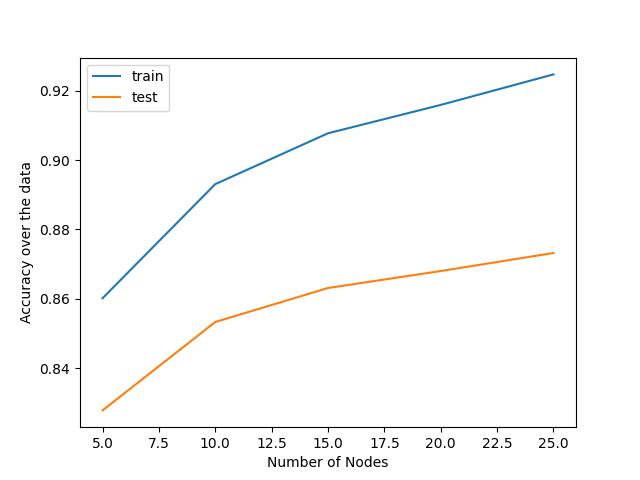
\includegraphics[width=\linewidth]{nn_b_plot.png}
  \caption{No. of Nodes vs Accuracy}
  \label{fig1B}
\end{figure}
\\
\subsection{Training Neural Network with adaptive learning rate}
The parameters for neural network training is :
\begin{enumerate}
\item Mini Batch Size : 100
\item No. of features : 784
\item Hidden Layers with no. of nodes : [5,10,15,20,25]
\item No. of target classes : 10
\item Learning Rate : Adaptive
\item Stopping Criteria ($\alpha$) : 1e-8
\item Maximum Iterations after which gradient descent stops : 1000
\end{enumerate}
The Accuracy and Confusion Matrix for is:
\vspace{3mm}
\hline
\begin{enumerate}
\item No. of hidden layer units = 5
\item Time to train the neural network = 175.3580424785614
\item Accuracy over Training data set = 0.8551
\item Accuracy over Test data set = 0.8227
\item Confusion Matrix over Training data set = 
\begin{equation}
  \begin{bmatrix}
 4530 &   29 &  144 &  191 &  114 &    9 &  819 &   17 &  136 &   11 \\
   16 & 5678 &   94 &  133 &   30 &    2 &   27 &    2 &   12 &    6 \\
  147 &    6 & 4445 &   32 &  872 &    2 &  437 &    0 &   59 &    0 \\
   99 &   74 &   92 & 4986 &  321 &    7 &  336 &   34 &   38 &   13 \\
   12 &    5 &  457 &   75 & 5068 &    2 &  352 &    0 &   29 &    0 \\
    5 &    0 &    2 &    1 &    2 & 5662 &    2 &  215 &   32 &   79 \\
  756 &    9 &  553 &   90 &  671 &    0 & 3796 &    9 &  112 &    4 \\
    1 &    0 &    1 &    0 &    1 &  125 &    1 & 5668 &   13 &  190 \\
   42 &    3 &   24 &   21 &   49 &    9 &   71 &   31 & 5745 &    5 \\
    3 &    2 &    0 &    0 &    0 &   45 &    1 &  218 &    3 & 5728 
  \end{bmatrix}
\end{equation}
\item Confusion Matrix over Test data set = 
\begin{equation}
  \begin{bmatrix}
737 & 4 & 22 & 37 & 15 & 3 & 140 & 7 & 33 & 2\\
4 & 941 & 17 & 29 & 4 & 0 & 2 & 0 & 2 & 1\\
42 & 2 & 705 & 10 & 161 & 0 & 77 & 0 & 3 & 0\\
19 & 25 & 16 & 784 & 63 & 0 & 79 & 3 & 10 & 1\\
1 & 2 & 105 & 16 & 791 & 0 & 75 & 0 & 10 & 0\\
1 & 0 & 1 & 1 & 0 & 906 & 0 & 51 & 14 & 26\\
118 & 1 & 112 & 24 & 142 & 0 & 569 & 1 & 31 & 2\\
0 & 0 & 0 & 0 & 0 & 29 & 0 & 931 & 1 & 39\\
13 & 0 & 3 & 4 & 15 & 3 & 17 & 11 & 934 & 0\\
3 & 0 & 0 & 0 & 0 & 12 & 1 & 55 & 0 & 929
  \end{bmatrix}
\end{equation}
\end{enumerate}
\hline
\begin{enumerate}
\item No. of hidden layer units = 10
\item Time to train the neural network = 221.94053149223328
\item Accuracy over Training data set = 0.8951666666666667
\item Accuracy over Test data set = 0.8496
\item Confusion Matrix over Training data set = 
\begin{equation}
  \begin{bmatrix}
5228 & 8 & 100 & 236 & 29 & 7 & 334 & 2 & 54 & 2\\
19 & 5835 & 13 & 104 & 12 & 1 & 13 & 0 & 2 & 1\\
71 & 9 & 4934 & 59 & 595 & 3 & 280 & 1 & 47 & 1\\
131 & 29 & 46 & 5522 & 161 & 2 & 95 & 1 & 11 & 2\\
12 & 8 & 439 & 175 & 5089 & 4 & 243 & 3 & 27 & 0\\
2 & 1 & 0 & 1 & 1 & 5819 & 3 & 116 & 16 & 41\\
747 & 16 & 555 & 198 & 491 & 1 & 3918 & 0 & 71 & 3\\
0 & 0 & 0 & 0 & 0 & 100 & 0 & 5744 & 12 & 144\\
20 & 3 & 27 & 25 & 24 & 15 & 61 & 11 & 5804 & 10\\
0 & 0 & 0 & 0 & 0 & 49 & 2 & 128 & 4 & 5817
  \end{bmatrix}
\end{equation}
\item Confusion Matrix over Test data set = 
\begin{equation}
  \begin{bmatrix}
808 & 3 & 15 & 56 & 9 & 0 & 94 & 1 & 13 & 1\\
4 & 957 & 5 & 27 & 4 & 0 & 3 & 0 & 0 & 0\\
19 & 3 & 769 & 12 & 121 & 1 & 69 & 2 & 4 & 0\\
32 & 13 & 13 & 874 & 35 & 0 & 26 & 0 & 6 & 1\\
0 & 2 & 114 & 39 & 769 & 3 & 62 & 0 & 11 & 0\\
0 & 0 & 1 & 1 & 0 & 924 & 0 & 46 & 5 & 23\\
139 & 2 & 123 & 54 & 110 & 2 & 552 & 0 & 17 & 1\\
0 & 0 & 0 & 0 & 0 & 28 & 0 & 945 & 0 & 27\\
1 & 1 & 8 & 5 & 8 & 4 & 19 & 5 & 948 & 1\\
0 & 0 & 0 & 0 & 0 & 12 & 1 & 37 & 0 & 950
  \end{bmatrix}
\end{equation}
\end{enumerate}
\hline
\begin{enumerate}
\item No. of hidden layer units = 15
\item Time to train the neural network = 264.362580537796
\item Accuracy over Training data set = 0.9064666666666666
\item Accuracy over Test data set = 0.8609
\item Confusion Matrix over Training data set = 
\begin{equation}
  \begin{bmatrix}
5211 & 11 & 74 & 136 & 30 & 5 & 480 & 1 & 50 & 2\\
17 & 5851 & 18 & 82 & 10 & 1 & 17 & 0 & 4 & 0\\
80 & 4 & 4908 & 46 & 568 & 3 & 347 & 0 & 44 & 0\\
143 & 22 & 32 & 5466 & 177 & 0 & 138 & 1 & 20 & 1\\
13 & 12 & 321 & 123 & 5175 & 3 & 327 & 1 & 24 & 1\\
3 & 0 & 0 & 0 & 0 & 5856 & 5 & 95 & 14 & 27\\
590 & 13 & 360 & 129 & 371 & 1 & 4451 & 1 & 83 & 1\\
0 & 0 & 0 & 2 & 0 & 61 & 0 & 5830 & 9 & 98\\
19 & 2 & 13 & 25 & 19 & 10 & 59 & 16 & 5834 & 3\\
0 & 0 & 0 & 0 & 0 & 29 & 0 & 161 & 4 & 5806
  \end{bmatrix}
\end{equation}
\item Confusion Matrix over Test data set = 
\begin{equation}
  \begin{bmatrix}
811 & 6 & 13 & 32 & 5 & 3 & 114 & 1 & 15 & 0\\
3 & 958 & 4 & 22 & 6 & 0 & 4 & 0 & 3 & 0\\
28 & 2 & 749 & 10 & 113 & 2 & 85 & 0 & 11 & 0\\
30 & 9 & 11 & 862 & 37 & 2 & 36 & 1 & 9 & 3\\
1 & 1 & 91 & 33 & 787 & 2 & 74 & 0 & 11 & 0\\
1 & 1 & 0 & 0 & 0 & 939 & 0 & 36 & 3 & 20\\
129 & 1 & 77 & 36 & 88 & 2 & 646 & 0 & 21 & 0\\
0 & 0 & 0 & 0 & 0 & 26 & 0 & 950 & 0 & 24\\
3 & 1 & 2 & 5 & 5 & 3 & 17 & 5 & 959 & 0\\
0 & 0 & 1 & 0 & 0 & 8 & 2 & 41 & 0 & 948
  \end{bmatrix}
\end{equation}
\end{enumerate}
\hline
\begin{enumerate}
\item No. of hidden layer units = 20
\item Time to train the neural network = 283.87608575820923
\item Accuracy over Training data set = 0.9173
\item Accuracy over Test data set = 0.866
\item Confusion Matrix over Training data set = 
\begin{equation}
  \begin{bmatrix}
5387 & 4 & 82 & 128 & 18 & 6 & 322 & 0 & 52 & 1\\
15 & 5850 & 14 & 94 & 8 & 0 & 14 & 0 & 5 & 0\\
81 & 5 & 5244 & 47 & 387 & 1 & 215 & 1 & 18 & 1\\
124 & 22 & 55 & 5535 & 148 & 0 & 97 & 0 & 19 & 0\\
15 & 10 & 433 & 153 & 5184 & 0 & 181 & 0 & 22 & 2\\
4 & 1 & 0 & 1 & 0 & 5887 & 2 & 70 & 11 & 24\\
599 & 11 & 457 & 127 & 305 & 0 & 4451 & 2 & 46 & 2\\
0 & 0 & 0 & 0 & 0 & 60 & 0 & 5821 & 11 & 108\\
21 & 2 & 29 & 18 & 17 & 2 & 45 & 20 & 5841 & 5\\
1 & 1 & 0 & 0 & 0 & 25 & 0 & 134 & 1 & 5838
  \end{bmatrix}
\end{equation}
\item Confusion Matrix over Test data set = 
\begin{equation}
  \begin{bmatrix}
819 & 2 & 15 & 37 & 5 & 1 & 106 & 0 & 15 & 0\\
3 & 958 & 1 & 27 & 6 & 0 & 4 & 0 & 1 & 0\\
23 & 2 & 819 & 10 & 84 & 1 & 52 & 1 & 8 & 0\\
26 & 8 & 18 & 885 & 25 & 0 & 31 & 1 & 6 & 0\\
0 & 1 & 119 & 43 & 779 & 0 & 53 & 0 & 5 & 0\\
0 & 1 & 0 & 0 & 0 & 943 & 0 & 34 & 4 & 18\\
146 & 0 & 116 & 32 & 88 & 0 & 599 & 0 & 19 & 0\\
0 & 0 & 0 & 0 & 0 & 28 & 0 & 943 & 0 & 29\\
4 & 1 & 3 & 7 & 5 & 2 & 15 & 4 & 959 & 0\\
0 & 1 & 0 & 0 & 0 & 11 & 0 & 31 & 1 & 956
  \end{bmatrix}
\end{equation}
\end{enumerate}
\hline
\begin{enumerate}
\item No. of hidden layer units = 25
\item Time to train the neural network = 350.8760907649994
\item Accuracy over Training data set = 0.9253166666666667
\item Accuracy over Test data set = 0.8741
\item Confusion Matrix over Training data set = 
\begin{equation}
  \begin{bmatrix}
5399 & 5 & 90 & 130 & 20 & 3 & 294 & 0 & 59 & 0\\
17 & 5872 & 11 & 81 & 7 & 0 & 10 & 0 & 2 & 0\\
73 & 3 & 5281 & 57 & 373 & 2 & 186 & 1 & 24 & 0\\
115 & 24 & 39 & 5586 & 143 & 0 & 79 & 0 & 14 & 0\\
18 & 5 & 357 & 135 & 5267 & 1 & 197 & 0 & 20 & 0\\
1 & 0 & 0 & 1 & 0 & 5905 & 1 & 68 & 9 & 15\\
515 & 18 & 347 & 125 & 285 & 4 & 4662 & 0 & 44 & 0\\
0 & 0 & 0 & 0 & 0 & 53 & 1 & 5825 & 10 & 111\\
15 & 4 & 31 & 21 & 15 & 2 & 32 & 14 & 5864 & 2\\
0 & 0 & 0 & 1 & 0 & 22 & 0 & 116 & 3 & 5858
  \end{bmatrix}
\end{equation}
\item Confusion Matrix over Test data set = 
\begin{equation}
  \begin{bmatrix}
832 & 2 & 16 & 37 & 3 & 3 & 91 & 0 & 16 & 0\\
4 & 962 & 2 & 25 & 3 & 0 & 3 & 0 & 1 & 0\\
18 & 1 & 805 & 15 & 97 & 2 & 56 & 0 & 6 & 0\\
32 & 7 & 17 & 892 & 28 & 1 & 19 & 0 & 4 & 0\\
0 & 2 & 107 & 39 & 792 & 0 & 54 & 0 & 6 & 0\\
1 & 0 & 0 & 1 & 1 & 945 & 0 & 28 & 2 & 22\\
128 & 0 & 105 & 34 & 70 & 1 & 644 & 0 & 18 & 0\\
0 & 0 & 0 & 0 & 0 & 20 & 0 & 949 & 1 & 30\\
0 & 1 & 7 & 5 & 1 & 5 & 11 & 4 & 966 & 0\\
0 & 0 & 0 & 0 & 0 & 11 & 0 & 34 & 1 & 954
  \end{bmatrix}
\end{equation}
\end{enumerate}
\begin{figure}[H]
  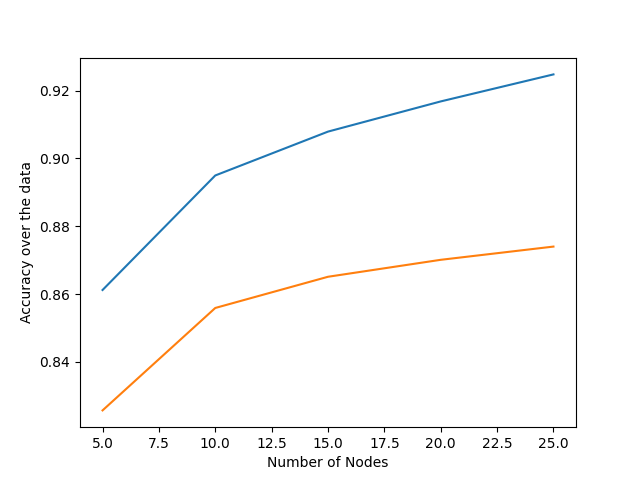
\includegraphics[width=\linewidth]{nn_c_plot.png}
  \caption{No. of Nodes vs Accuracy}
  \label{fig1B}
\end{figure}
\\

\subsection{Sigmoid and ReLu as activation Functions}
Using Sigmoid as Activation Function, the accuracy and confusion matrices are:
\begin{enumerate}
\item No. of hidden layer units = [100, 100]
\item Time to train the neural network = 904.3589193820953
\item Accuracy over Training data set = 0.9696
\item Accuracy over Test data set = 0.8848
\item Confusion Matrix over Training data set = 
\begin{equation}
  \begin{bmatrix}
5790 & 8 & 60 & 38 & 10 & 3 & 58 & 0 & 31 & 2\\
17 & 5922 & 5 & 36 & 6 & 1 & 6 & 1 & 4 & 2\\
66 & 1 & 5701 & 31 & 122 & 2 & 67 & 0 & 10 & 0\\
48 & 5 & 40 & 5806 & 53 & 0 & 38 & 0 & 10 & 0\\
25 & 5 & 139 & 74 & 5686 & 1 & 58 & 0 & 12 & 0\\
0 & 1 & 1 & 1 & 0 & 5970 & 0 & 20 & 4 & 3\\
172 & 12 & 138 & 69 & 93 & 0 & 5502 & 2 & 12 & 0\\
0 & 0 & 0 & 0 & 0 & 11 & 0 & 5942 & 3 & 44\\
14 & 3 & 17 & 14 & 13 & 1 & 5 & 6 & 5922 & 5\\
0 & 0 & 0 & 2 & 0 & 8 & 0 & 55 & 0 & 5935
  \end{bmatrix}
\end{equation}
\item Confusion Matrix over Test data set = 
\begin{equation}
  \begin{bmatrix}
855 & 1 & 17 & 17 & 4 & 4 & 91 & 0 & 11 & 0\\
8 & 968 & 0 & 14 & 2 & 0 & 7 & 0 & 1 & 0\\
17 & 2 & 834 & 12 & 76 & 0 & 56 & 0 & 3 & 0\\
32 & 6 & 23 & 889 & 28 & 0 & 18 & 0 & 4 & 0\\
1 & 1 & 104 & 34 & 793 & 1 & 63 & 0 & 3 & 0\\
0 & 0 & 0 & 1 & 0 & 954 & 0 & 26 & 1 & 18\\
135 & 3 & 80 & 24 & 67 & 0 & 678 & 0 & 13 & 0\\
0 & 0 & 0 & 0 & 0 & 22 & 0 & 955 & 0 & 23\\
6 & 0 & 5 & 5 & 3 & 2 & 11 & 5 & 963 & 0\\
0 & 0 & 0 & 0 & 0 & 10 & 0 & 30 & 1 & 959
  \end{bmatrix}
\end{equation}
\end{enumerate}
\hline
\vspace{3mm}
Using ReLu as Activation Function, the accuracy and confusion matrices are:
\begin{enumerate}
\item No. of hidden layer units = [100, 100]
\item Time to train the neural network = 899.413823712596
\item Accuracy over Training data set = 0.9823833333333334
\item Accuracy over Test data set = 0.8827
\item Confusion Matrix over Training data set = 
\begin{equation}
  \begin{bmatrix}
5831 & 6 & 31 & 28 & 16 & 2 & 69 & 0 & 17 & 0\\
7 & 5949 & 3 & 14 & 9 & 0 & 17 & 0 & 1 & 0\\
22 & 3 & 5810 & 32 & 47 & 0 & 73 & 0 & 12 & 1\\
17 & 4 & 19 & 5887 & 16 & 0 & 50 & 0 & 7 & 0\\
8 & 4 & 30 & 24 & 5886 & 2 & 41 & 0 & 5 & 0\\
0 & 0 & 1 & 2 & 0 & 5975 & 0 & 14 & 5 & 3\\
55 & 13 & 69 & 36 & 60 & 1 & 5747 & 4 & 14 & 1\\
0 & 0 & 0 & 0 & 0 & 9 & 0 & 5952 & 4 & 35\\
4 & 3 & 9 & 3 & 9 & 3 & 15 & 14 & 5937 & 3\\
0 & 1 & 0 & 0 & 0 & 3 & 0 & 26 & 1 & 5969
  \end{bmatrix}
\end{equation}
\item Confusion Matrix over Test data set = 
\begin{equation}
  \begin{bmatrix}
807 & 1 & 19 & 26 & 5 & 2 & 132 & 0 & 8 & 0\\
5 & 968 & 3 & 12 & 6 & 1 & 4 & 0 & 1 & 0\\
21 & 3 & 809 & 9 & 79 & 2 & 71 & 0 & 5 & 1\\
23 & 8 & 11 & 884 & 34 & 1 & 35 & 0 & 4 & 0\\
1 & 1 & 83 & 33 & 820 & 1 & 58 & 0 & 3 & 0\\
2 & 0 & 0 & 1 & 0 & 948 & 2 & 31 & 3 & 13\\
116 & 2 & 70 & 20 & 65 & 0 & 718 & 0 & 8 & 1\\
0 & 0 & 0 & 0 & 0 & 19 & 0 & 962 & 0 & 19\\
4 & 0 & 5 & 8 & 8 & 3 & 9 & 7 & 956 & 0\\
0 & 0 & 0 & 1 & 0 & 10 & 1 & 33 & 0 & 955
  \end{bmatrix}
\end{equation}
\end{enumerate}


\subsection{Varying the number of hidden layers}
Varying the number of hidden layers increases the size of the set of hypothesis functions that neural network can approximate. The number of units per hidden layer is 50. The no. of hidden layers are varied from 2 to 5. \\
\textbf{Using sigmoid as activation function:}
\begin{enumerate}
\item No. of hidden layer units = [50, 50]
\item Time to train the neural network = 585.0355925559998
\item Accuracy over Training data set = 0.9571833333333334
\item Accuracy over Test data set = 0.8778
\item Confusion Matrix over Training data set = 
\begin{equation}
  \begin{bmatrix}
5598 & 8 & 65 & 65 & 21 & 2 & 211 & 0 & 28 & 2\\
13 & 5909 & 2 & 50 & 13 & 1 & 9 & 0 & 2 & 1\\
62 & 3 & 5377 & 40 & 321 & 1 & 181 & 0 & 14 & 1\\
37 & 6 & 32 & 5735 & 91 & 0 & 90 & 1 & 8 & 0\\
11 & 3 & 114 & 94 & 5630 & 0 & 137 & 0 & 11 & 0\\
1 & 1 & 0 & 1 & 0 & 5972 & 2 & 18 & 2 & 3\\
193 & 14 & 106 & 84 & 153 & 1 & 5430 & 2 & 17 & 0\\
0 & 0 & 0 & 0 & 0 & 12 & 0 & 5948 & 4 & 36\\
15 & 4 & 11 & 13 & 20 & 2 & 16 & 11 & 5904 & 4\\
0 & 0 & 1 & 0 & 0 & 10 & 0 & 58 & 3 & 5928
  \end{bmatrix}
\end{equation}
\item Confusion Matrix over Test data set = 
\begin{equation}
  \begin{bmatrix}
818 & 1 & 15 & 30 & 4 & 3 & 118 & 0 & 11 & 0\\
6 & 961 & 6 & 22 & 3 & 0 & 1 & 0 & 1 & 0\\
15 & 2 & 762 & 13 & 120 & 1 & 86 & 0 & 1 & 0\\
29 & 5 & 19 & 883 & 29 & 0 & 32 & 0 & 3 & 0\\
1 & 2 & 71 & 32 & 828 & 0 & 60 & 1 & 5 & 0\\
0 & 0 & 0 & 2 & 0 & 950 & 0 & 26 & 2 & 20\\
110 & 1 & 70 & 28 & 77 & 0 & 703 & 0 & 11 & 0\\
0 & 0 & 0 & 0 & 0 & 24 & 0 & 955 & 0 & 21\\
3 & 0 & 4 & 7 & 3 & 2 & 10 & 6 & 965 & 0\\
0 & 0 & 0 & 0 & 0 & 13 & 1 & 33 & 0 & 953
  \end{bmatrix}
\end{equation}
\end{enumerate}
\hline
\begin{enumerate}
\item No. of hidden layer units = [50, 50, 50]
\item Time to train the neural network = 732.591703414917
\item Accuracy over Training data set = 0.9567333333333333
\item Accuracy over Test data set = 0.8744
\item Confusion Matrix over Training data set = 
\begin{equation}
  \begin{bmatrix}
5729 & 4 & 95 & 52 & 33 & 3 & 58 & 0 & 25 & 1\\
19 & 5917 & 12 & 33 & 15 & 0 & 3 & 0 & 1 & 0\\
63 & 7 & 5642 & 30 & 194 & 2 & 50 & 1 & 9 & 2\\
58 & 12 & 44 & 5708 & 146 & 0 & 25 & 0 & 4 & 3\\
16 & 8 & 200 & 51 & 5675 & 0 & 42 & 0 & 6 & 2\\
4 & 0 & 0 & 2 & 0 & 5957 & 1 & 25 & 3 & 8\\
329 & 9 & 339 & 47 & 283 & 3 & 4974 & 0 & 14 & 2\\
1 & 0 & 0 & 0 & 0 & 10 & 0 & 5941 & 0 & 48\\
25 & 6 & 27 & 7 & 22 & 1 & 7 & 1 & 5900 & 4\\
0 & 0 & 0 & 0 & 1 & 7 & 0 & 29 & 2 & 5961
  \end{bmatrix}
\end{equation}
\item Confusion Matrix over Test data set = 
\begin{equation}
  \begin{bmatrix}
847 & 3 & 21 & 29 & 9 & 0 & 81 & 0 & 10 & 0\\
11 & 970 & 2 & 12 & 2 & 0 & 2 & 0 & 1 & 0\\
20 & 3 & 828 & 12 & 92 & 0 & 43 & 0 & 1 & 1\\
43 & 9 & 20 & 859 & 45 & 1 & 19 & 0 & 4 & 0\\
0 & 2 & 118 & 23 & 820 & 0 & 33 & 1 & 2 & 1\\
0 & 0 & 0 & 0 & 0 & 944 & 0 & 30 & 2 & 24\\
150 & 1 & 101 & 26 & 99 & 0 & 613 & 0 & 10 & 0\\
0 & 0 & 0 & 0 & 0 & 18 & 0 & 945 & 0 & 37\\
4 & 1 & 6 & 3 & 8 & 7 & 10 & 4 & 956 & 1\\
0 & 0 & 0 & 0 & 0 & 9 & 0 & 28 & 1 & 962
  \end{bmatrix}
\end{equation}
\end{enumerate}
\hline
\begin{enumerate}
\item No. of hidden layer units = [50, 50, 50, 50]
\item Time to train the neural network = 816.7182228565216
\item Accuracy over Training data set = 0.9506333333333333
\item Accuracy over Test data set = 0.8663
\item Confusion Matrix over Training data set = 
\begin{equation}
  \begin{bmatrix}
5720 & 9 & 86 & 54 & 14 & 16 & 84 & 0 & 17 & 0\\
12 & 5911 & 20 & 37 & 5 & 3 & 7 & 1 & 4 & 0\\
64 & 3 & 5692 & 29 & 124 & 5 & 76 & 0 & 7 & 0\\
37 & 4 & 61 & 5802 & 51 & 1 & 36 & 0 & 8 & 0\\
18 & 10 & 459 & 70 & 5376 & 3 & 59 & 0 & 5 & 0\\
0 & 0 & 1 & 0 & 0 & 5976 & 1 & 16 & 4 & 2\\
422 & 11 & 526 & 108 & 126 & 7 & 4792 & 0 & 7 & 1\\
0 & 0 & 0 & 0 & 0 & 34 & 0 & 5939 & 4 & 23\\
27 & 5 & 39 & 12 & 8 & 8 & 7 & 7 & 5879 & 8\\
0 & 2 & 1 & 0 & 0 & 9 & 0 & 37 & 0 & 5951
  \end{bmatrix}
\end{equation}
\item Confusion Matrix over Test data set = 
\begin{equation}
  \begin{bmatrix}
848 & 1 & 26 & 31 & 6 & 4 & 78 & 0 & 6 & 0\\
5 & 966 & 4 & 16 & 3 & 1 & 5 & 0 & 0 & 0\\
17 & 0 & 874 & 11 & 52 & 2 & 42 & 0 & 2 & 0\\
37 & 12 & 22 & 870 & 35 & 1 & 21 & 0 & 2 & 0\\
1 & 1 & 172 & 36 & 733 & 0 & 53 & 0 & 4 & 0\\
1 & 0 & 0 & 0 & 0 & 948 & 0 & 31 & 2 & 18\\
159 & 1 & 124 & 39 & 71 & 2 & 589 & 0 & 15 & 0\\
0 & 0 & 0 & 0 & 0 & 32 & 0 & 941 & 0 & 27\\
2 & 0 & 8 & 6 & 8 & 10 & 6 & 4 & 954 & 2\\
0 & 0 & 0 & 0 & 0 & 17 & 1 & 42 & 0 & 940
  \end{bmatrix}
\end{equation}
\end{enumerate}
\hline
\begin{enumerate}
\item No. of hidden layer units = [50, 50, 50, 50, 50]
\item Time to train the neural network = 921.581799030304
\item Accuracy over Training data set = 0.9577833333333333
\item Accuracy over Test data set = 0.8676
\item Confusion Matrix over Training data set = 
\begin{equation}
  \begin{bmatrix}
5670 & 7 & 33 & 75 & 33 & 17 & 125 & 0 & 40 & 0\\
56 & 5783 & 40 & 64 & 12 & 2 & 39 & 1 & 2 & 1\\
44 & 2 & 5571 & 47 & 191 & 4 & 127 & 0 & 14 & 0\\
61 & 2 & 33 & 5740 & 70 & 5 & 75 & 0 & 13 & 1\\
29 & 10 & 144 & 122 & 5542 & 2 & 145 & 0 & 6 & 0\\
1 & 1 & 1 & 0 & 1 & 5965 & 1 & 20 & 7 & 3\\
226 & 7 & 102 & 69 & 126 & 2 & 5452 & 0 & 15 & 1\\
0 & 0 & 0 & 0 & 0 & 13 & 0 & 5940 & 12 & 35\\
18 & 3 & 29 & 18 & 20 & 20 & 40 & 3 & 5846 & 3\\
0 & 0 & 2 & 1 & 0 & 7 & 0 & 29 & 3 & 5958\\
  \end{bmatrix}
\end{equation}
\item Confusion Matrix over Test data set = 
\begin{equation}
  \begin{bmatrix}
805 & 1 & 23 & 36 & 6 & 1 & 120 & 0 & 8 & 0\\
7 & 944 & 7 & 29 & 5 & 0 & 7 & 0 & 1 & 0\\
21 & 0 & 800 & 8 & 84 & 0 & 86 & 0 & 1 & 0\\
38 & 16 & 8 & 862 & 26 & 1 & 46 & 0 & 3 & 0\\
5 & 0 & 98 & 30 & 782 & 0 & 75 & 0 & 10 & 0\\
0 & 1 & 0 & 0 & 0 & 941 & 0 & 36 & 8 & 14\\
120 & 0 & 68 & 33 & 84 & 2 & 683 & 0 & 10 & 0\\
0 & 0 & 0 & 0 & 0 & 21 & 0 & 954 & 0 & 25\\
0 & 0 & 4 & 6 & 9 & 12 & 12 & 3 & 951 & 3\\
0 & 0 & 0 & 1 & 0 & 11 & 0 & 33 & 1 & 954\\
  \end{bmatrix}
\end{equation}
\end{enumerate}
\hline
\vspace{3mm}
\textbf{Using ReLu as activation function}
\begin{enumerate}
\item No. of hidden layer units = [50, 50]
\item Time to train the neural network = 601.0700619220734
\item Accuracy over Training data set = 0.9542333333333334
\item Accuracy over Test data set = 0.8689
\item Confusion Matrix over Training data set = 
\begin{equation}
  \begin{bmatrix}
5402 & 12 & 30 & 47 & 23 & 2 & 445 & 1 & 38 & 0\\
6 & 5905 & 6 & 50 & 9 & 6 & 11 & 1 & 5 & 1\\
18 & 2 & 5227 & 28 & 269 & 1 & 446 & 1 & 8 & 0\\
12 & 5 & 22 & 5746 & 109 & 0 & 97 & 2 & 7 & 0\\
3 & 5 & 96 & 53 & 5630 & 1 & 197 & 0 & 14 & 1\\
0 & 2 & 1 & 1 & 0 & 5967 & 2 & 17 & 4 & 6\\
96 & 9 & 79 & 65 & 135 & 0 & 5584 & 0 & 28 & 4\\
0 & 0 & 0 & 0 & 0 & 5 & 0 & 5921 & 8 & 66\\
5 & 5 & 10 & 10 & 24 & 1 & 27 & 10 & 5904 & 4\\
0 & 0 & 0 & 0 & 0 & 5 & 0 & 27 & 0 & 5968
  \end{bmatrix}
\end{equation}
\item Confusion Matrix over Test data set = 
\begin{equation}
  \begin{bmatrix}
773 & 3 & 9 & 23 & 8 & 2 & 171 & 0 & 11 & 0\\
2 & 966 & 4 & 20 & 3 & 0 & 3 & 0 & 2 & 0\\
12 & 2 & 747 & 9 & 105 & 2 & 119 & 1 & 3 & 0\\
24 & 17 & 8 & 856 & 49 & 2 & 37 & 1 & 5 & 1\\
4 & 1 & 75 & 33 & 803 & 0 & 79 & 0 & 4 & 1\\
0 & 0 & 0 & 2 & 0 & 940 & 1 & 31 & 6 & 20\\
84 & 4 & 54 & 21 & 65 & 2 & 755 & 0 & 14 & 1\\
0 & 0 & 0 & 0 & 0 & 18 & 0 & 944 & 0 & 38\\
4 & 3 & 8 & 5 & 7 & 4 & 13 & 6 & 950 & 0\\
1 & 0 & 0 & 1 & 0 & 11 & 1 & 31 & 0 & 955
  \end{bmatrix}
\end{equation}
\end{enumerate}
\hline
\begin{enumerate}
\item No. of hidden layer units = [50, 50, 50]
\item Time to train the neural network = 722.5276672840118
\item Accuracy over Training data set = 0.8903
\item Accuracy over Test data set = 0.8004
\item Confusion Matrix over Training data set = 
\begin{equation}
  \begin{bmatrix}
5836 & 6 & 30 & 30 & 15 & 2 & 56 & 0 & 25 & 0\\
14 & 5935 & 3 & 26 & 11 & 1 & 6 & 1 & 3 & 0\\
41 & 3 & 5706 & 20 & 124 & 3 & 85 & 3 & 15 & 0\\
42 & 12 & 18 & 5840 & 48 & 1 & 34 & 0 & 5 & 0\\
13 & 7 & 144 & 41 & 5718 & 0 & 67 & 0 & 10 & 0\\
2 & 3 & 0 & 1 & 0 & 5976 & 0 & 17 & 1 & 0\\
171 & 13 & 83 & 36 & 79 & 2 & 5589 & 1 & 26 & 0\\
0 & 0 & 0 & 0 & 1 & 15 & 0 & 5977 & 5 & 2\\
11 & 2 & 9 & 7 & 12 & 4 & 11 & 5 & 5939 & 0\\
23 & 5 & 30 & 10 & 443 & 1851 & 21 & 2287 & 428 & 902
  \end{bmatrix}
\end{equation}
\item Confusion Matrix over Test data set = 
\begin{equation}
  \begin{bmatrix}
850 & 3 & 14 & 25 & 1 & 0 & 96 & 2 & 9 & 0\\
9 & 965 & 4 & 13 & 6 & 0 & 3 & 0 & 0 & 0\\
22 & 0 & 798 & 8 & 79 & 0 & 84 & 1 & 8 & 0\\
35 & 6 & 11 & 876 & 39 & 0 & 27 & 0 & 6 & 0\\
4 & 2 & 107 & 30 & 792 & 0 & 60 & 0 & 5 & 0\\
2 & 0 & 0 & 1 & 1 & 961 & 1 & 30 & 4 & 0\\
148 & 5 & 65 & 23 & 80 & 0 & 668 & 0 & 11 & 0\\
0 & 0 & 1 & 0 & 0 & 27 & 0 & 971 & 1 & 0\\
3 & 1 & 8 & 10 & 2 & 1 & 9 & 7 & 959 & 0\\
5 & 1 & 4 & 1 & 72 & 309 & 6 & 375 & 63 & 164
  \end{bmatrix}
\end{equation}
\end{enumerate}
\hline
\begin{enumerate}

\item No. of hidden layer units = [50, 50, 50, 50]
\item Time to train the neural network = 821.6736297607422
\item Accuracy over Training data set = 0.9751833333333333
\item Accuracy over Test data set = 0.8735
\item Confusion Matrix over Training data set = 
\begin{equation}
  \begin{bmatrix}
5761 & 6 & 31 & 40 & 13 & 1 & 114 & 1 & 32 & 1\\
7 & 5922 & 6 & 39 & 6 & 0 & 17 & 0 & 2 & 1\\
26 & 5 & 5711 & 27 & 163 & 0 & 58 & 0 & 10 & 0\\
18 & 9 & 14 & 5866 & 36 & 1 & 50 & 0 & 6 & 0\\
12 & 4 & 73 & 36 & 5804 & 0 & 61 & 0 & 8 & 2\\
0 & 1 & 0 & 1 & 0 & 5966 & 0 & 21 & 2 & 9\\
99 & 7 & 79 & 35 & 139 & 3 & 5619 & 0 & 17 & 2\\
0 & 0 & 1 & 1 & 0 & 4 & 0 & 5965 & 2 & 27\\
11 & 5 & 11 & 14 & 15 & 1 & 9 & 3 & 5931 & 0\\
0 & 0 & 0 & 0 & 0 & 1 & 0 & 32 & 1 & 5966
  \end{bmatrix}
\end{equation}
\item Confusion Matrix over Test data set = 
\begin{equation}
  \begin{bmatrix}
806 & 1 & 16 & 27 & 5 & 1 & 131 & 2 & 11 & 0\\
8 & 959 & 3 & 21 & 5 & 0 & 3 & 0 & 0 & 1\\
17 & 0 & 782 & 18 & 103 & 1 & 74 & 0 & 5 & 0\\
33 & 10 & 14 & 857 & 35 & 0 & 45 & 0 & 4 & 2\\
2 & 0 & 85 & 36 & 819 & 2 & 52 & 0 & 4 & 0\\
0 & 0 & 0 & 0 & 0 & 939 & 1 & 34 & 4 & 22\\
107 & 2 & 66 & 23 & 89 & 1 & 699 & 0 & 13 & 0\\
0 & 0 & 0 & 0 & 0 & 20 & 0 & 959 & 1 & 20\\
4 & 1 & 3 & 13 & 5 & 6 & 8 & 5 & 955 & 0\\
0 & 0 & 1 & 1 & 0 & 8 & 0 & 29 & 1 & 960\\
  \end{bmatrix}
\end{equation}
\end{enumerate}
\hline
\begin{enumerate}
\item No. of hidden layer units = [50, 50, 50, 50, 50]
\item Time to train the neural network = 861.6063125133514
\item Accuracy over Training data set = 0.9791
\item Accuracy over Test data set = 0.8803
\item Confusion Matrix over Training data set = 
\begin{equation}
  \begin{bmatrix}
5879 & 7 & 30 & 39 & 4 & 2 & 28 & 1 & 9 & 1\\
9 & 5945 & 8 & 27 & 5 & 2 & 2 & 0 & 2 & 0\\
43 & 4 & 5780 & 33 & 88 & 1 & 40 & 0 & 11 & 0\\
39 & 1 & 14 & 5888 & 30 & 1 & 21 & 1 & 5 & 0\\
18 & 5 & 90 & 55 & 5789 & 0 & 39 & 0 & 4 & 0\\
0 & 0 & 3 & 1 & 1 & 5973 & 1 & 13 & 3 & 5\\
171 & 10 & 67 & 53 & 53 & 2 & 5634 & 1 & 6 & 3\\
0 & 0 & 0 & 0 & 0 & 6 & 0 & 5959 & 3 & 32\\
12 & 2 & 13 & 13 & 4 & 1 & 9 & 0 & 5945 & 1\\
0 & 0 & 0 & 0 & 0 & 9 & 0 & 37 & 0 & 5954
  \end{bmatrix}
\end{equation}
\item Confusion Matrix over Test data set = 
\begin{equation}
  \begin{bmatrix}
853 & 2 & 15 & 23 & 3 & 1 & 95 & 0 & 8 & 0\\
3 & 968 & 2 & 18 & 6 & 0 & 2 & 0 & 0 & 1\\
22 & 1 & 812 & 15 & 76 & 1 & 66 & 1 & 6 & 0\\
33 & 9 & 11 & 886 & 27 & 0 & 27 & 0 & 7 & 0\\
2 & 3 & 81 & 41 & 809 & 1 & 57 & 2 & 4 & 0\\
2 & 0 & 0 & 3 & 1 & 947 & 0 & 29 & 2 & 16\\
144 & 2 & 73 & 30 & 79 & 1 & 658 & 0 & 12 & 1\\
0 & 0 & 0 & 0 & 0 & 24 & 0 & 949 & 1 & 26\\
13 & 1 & 5 & 6 & 7 & 3 & 4 & 2 & 958 & 1\\
0 & 0 & 0 & 0 & 0 & 12 & 1 & 24 & 0 & 963
  \end{bmatrix}
\end{equation}
\end{enumerate}
\begin{figure}[H]
  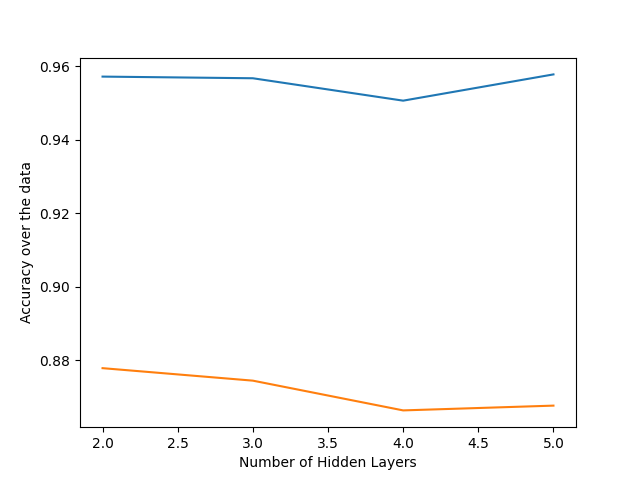
\includegraphics[width=\linewidth]{e_sigmoid_plot.png}
  \caption{No. of Hidden Layers vs Accuracy (Sigmoid)}
  \label{fig1B}
\end{figure}
\begin{figure}[H]
  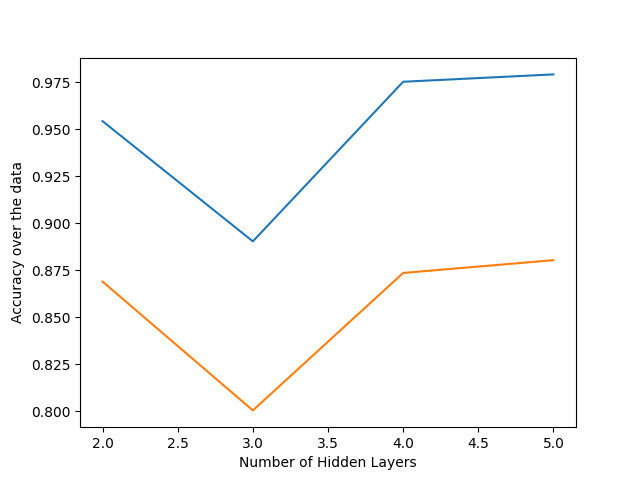
\includegraphics[width=\linewidth]{e_ReLu_plot.png}
  \caption{No. of Hidden Layers vs Accuracy (ReLu)}
  \label{fig1B}
\end{figure}
\subsection{Training the network using BCE objective function}
Considering the backpropagation was programmed to implement a stochastic gradient descent on a desired cost function $J$, we can formulate the following :

Let the output of neurons be $\mathcal{O}_j$ and $\psi$ be the activation function.
\begin{equation*}
    \centering
    \begin{split}        
        \delta_j = \frac{\partial J}{\partial \mathcal{O}_j}\frac{\partial \mathcal{O}_j}{\partial net_j} = \begin{cases}
        \frac{\partial J(\mathcal{O}_j,y)}{\partial \mathcal{O}_j}\frac{\partial\psi(net_j)}{\partial net_j} & \text{if $j$ is and output neuron } \\
        (\sum_{l\in L} w_{jl}\delta_l)\frac{\partial\psi(net_j)}{\partial net_j} & \text{if $j$ is and inner neuron }\\
    \end{cases}
    \end{split}
\end{equation*}
The only change to implement gradient descent on binary cross entropy loss will be in the $\delta_j$ calculation at the output layer, where ${\partial J(\mathcal{O}_j,y)}/{\partial \mathcal{O}_j}$ will now be evaluated as follows.
\begin{equation}
        J(\mathcal{O},y) = -\sum_{j = 1}^{C}{y_jlog(\mathcal{O}_j) + (1-y_j)log(1-\mathcal{O}_j)}
        \end{equation}
    \begin{equation*}
             \frac{\partial J(\mathcal{O},y)}{\partial\mathcal{O}_j} = \frac{\mathcal{O}_j-y_j}{\mathcal{O}_j(1-\mathcal{O}_j)}
    \end{equation*}
        
    \begin{equation*}
         \frac{\partial J(\mathcal{O}_j,y)}{\partial \mathcal{O}_j}\frac{\partial\psi(net_j)}{\partial net_j} = \mathcal{O}_j-y_j
    \end{equation*}
        


\begin{enumerate}
\item No. of hidden layer units = [50, 50, 50]
% \item Time to train the neural network = 861.6063125133514
\item Accuracy over Training data set = 0.9637
\item Accuracy over Test data set = 0.8827
\item Confusion Matrix over Training data set = 
\begin{equation}
  \begin{bmatrix}
5871 & 9 & 34 & 39 & 4 & 2 & 28 & 1 & 9 & 1\\
9 & 5951 & 4 & 23 & 5 & 2 & 2 & 0 & 1 & 0\\
41 & 3 & 5784 & 33 & 83 & 5 & 40 & 0 & 11 & 0\\
37 & 3 & 9 & 5888 & 30 & 1 & 22 & 4 & 7 & 0\\
17 & 5 & 89 & 55 & 5793 & 0 & 37 & 0 & 3 & 0\\
0 & 0 & 2 & 1 & 1 & 5975 & 1 & 13 & 3 & 4\\
169 & 9 & 69 & 53 & 54 & 3 & 5631 & 1 & 7 & 4\\
0 & 0 & 0 & 0 & 0 & 5 & 0 & 5961 & 3 & 31\\
11 & 2 & 14 & 13 & 3 & 2 & 10 & 0 & 5941 & 3\\
0 & 1 & 0 & 0 & 1 & 7 & 0 & 35 & 0 & 5959
  \end{bmatrix}
\end{equation}
\item Confusion Matrix over Test data set = 
\begin{equation}
  \begin{bmatrix}
851 & 2 & 15 & 25 & 3 & 1 & 95 & 0 & 8 & 0\\
3 & 969 & 2 & 18 & 6 & 0 & 2 & 0 & 0 & 2\\
23 & 1 & 809 & 15 & 76 & 2 & 67 & 1 & 6 & 0\\
33 & 9 & 11 & 889 & 27 & 0 & 25 & 0 & 6 & 0\\
1 & 3 & 80 & 41 & 811 & 1 & 57 & 2 & 4 & 0\\
2 & 0 & 1 & 3 & 2 & 941 & 0 & 231 & 3 & 16\\
144 & 2 & 73 & 30 & 79 & 1 & 659 & 0 & 13 & 1\\
0 & 0 & 0 & 0 & 0 & 25 & 0 & 947 & 1 & 27\\
12 & 1 & 5 & 6 & 7 & 3 & 4 & 2 & 959 & 1\\
0 & 0 & 0 & 0 & 0 & 11 & 1 & 23 & 0 & 965
  \end{bmatrix}
\end{equation}
\end{enumerate}
\subsection{Training the network using MLPClassifier}
The MLPClassifier from scikit-learn library to implement a neural network with 2 hidden layers with 100 units each. The activation function used ReLu and MLPClassifier by default uses binary cross entropy loss. The accuracies are:
\begin{enumerate}
\item No. of hidden layer units = [100,100]
% \item Time to train the neural network = 861.6063125133514
\item Accuracy over Training data set = 0.9886
\item Accuracy over Test data set = 0.8925
\item Confusion Matrix over Training data set = 
\begin{equation}
  \begin{bmatrix}
5871 & 9 & 34 & 39 & 4 & 2 & 28 & 1 & 9 & 1\\
9 & 5951 & 4 & 23 & 5 & 2 & 2 & 0 & 1 & 0\\
41 & 3 & 5784 & 33 & 83 & 5 & 40 & 0 & 11 & 0\\
37 & 3 & 9 & 5888 & 30 & 1 & 22 & 4 & 7 & 0\\
17 & 5 & 89 & 55 & 5793 & 0 & 37 & 0 & 3 & 0\\
0 & 0 & 2 & 1 & 1 & 5975 & 1 & 13 & 3 & 4\\
169 & 9 & 69 & 53 & 54 & 3 & 5631 & 1 & 7 & 4\\
0 & 0 & 0 & 0 & 0 & 5 & 0 & 5961 & 3 & 31\\
11 & 2 & 14 & 13 & 3 & 2 & 10 & 0 & 5941 & 3\\
0 & 1 & 0 & 0 & 1 & 7 & 0 & 35 & 0 & 5959
  \end{bmatrix}
\end{equation}
\item Confusion Matrix over Test data set = 
\begin{equation}
  \begin{bmatrix}
851 & 2 & 15 & 25 & 3 & 1 & 95 & 0 & 8 & 0\\
3 & 969 & 2 & 18 & 6 & 0 & 2 & 0 & 0 & 2\\
23 & 1 & 809 & 15 & 76 & 2 & 67 & 1 & 6 & 0\\
33 & 9 & 11 & 889 & 27 & 0 & 25 & 0 & 6 & 0\\
1 & 3 & 80 & 41 & 811 & 1 & 57 & 2 & 4 & 0\\
2 & 0 & 1 & 3 & 2 & 941 & 0 & 231 & 3 & 16\\
144 & 2 & 73 & 30 & 79 & 1 & 659 & 0 & 13 & 1\\
0 & 0 & 0 & 0 & 0 & 25 & 0 & 947 & 1 & 27\\
12 & 1 & 5 & 6 & 7 & 3 & 4 & 2 & 959 & 1\\
0 & 0 & 0 & 0 & 0 & 11 & 1 & 23 & 0 & 965
  \end{bmatrix}
\end{equation}
\end{enumerate}
\end{document}